% !TEX root = userguide_jp.tex
%----------------------------------------------------------
\chapter{ファイル仕様}

%----------------------------------------------------------
\section{スタンダードモード用入力ファイル}
\label{Ch:HowToStandard}

スタンダードモード用入力ファイルは次のような格好をしています。

\begin{minipage}{10cm}
\begin{screen}
\begin{verbatim}
W = 2
 L = 4
 model = "spin"

 lattice = "triangular lattice"
//mu = 1.0
// t = -1.0
// t' = -0.5
// U = 8.0
//V = 4.0
//V'=2.0
J = -1.0
J'=-0.5
// nelec = 8
2Sz = 0
\end{verbatim}
\end{screen}
\end{minipage}

大まかなルールは次のとおりです。
\begin{itemize}
\item 各行にはひと組ずつキーワード(\verb|=|の前)と
  パラメーター(\verb|=|の後)が書かれており間は\verb|=|で区切られています。
\item 各キーワードは順不同に記述できます。
\item 空白行、または\verb|//|で始まる行(コメントアウト)は読み飛ばされます。
\item 各キーワード、パラメーターの大文字$\cdot$小文字は区別されません。
  ダブルクオート、空白は無視されます。
\item 必ず指定しなければいけないパラメーター、
  指定しない場合デフォルト値が使われるパラメーター、
  (他のパラメーターの組み合わせによっては)使われないパラメーターが存在します。
  使われないパラメーターが指定された場合にはプログラムは終了し、
  入力ファイルをチェックするようにというメッセージが表示されます。
\end{itemize}

次に各キーワードの説明をします。

\subsection{計算の種類に関する必須パラメーター}

\begin{itemize}

\item \verb|model|

{\bf 形式 :} 文字列(\verb|"Fermion Hubbard"|, \verb|"Spin"|, \verb|"Kondo Lattice"|, 
\verb|"Fermion HubbardGC"|, \verb|"SpinGC"|, \verb|"Kondo LatticeGC"|のいずれか)

{\bf 説明 :} 計算対象の模型を指定します。上記の文字列はそれぞれ
カノニカル集団のフェルミ粒子Hubbard模型
\begin{align}
H = - \mu \sum_{i \sigma} c^\dagger_{i \sigma} c_{i \sigma} 
- \sum_{i \neq j \sigma} t_{i j} c^\dagger_{i \sigma} c_{j \sigma} 
+ \sum_{i} U n_{i \uparrow} n_{i \downarrow}
+ \sum_{i \neq j} V_{i j} n_{i} n_{j},
\label{fml4_1_hubbard}
\end{align}
同じくカノニカル集団のスピン模型 ($\{\sigma_1, \sigma_2\}={x, y, z}$)
\begin{align}
H &= -h \sum_{i} S_{i z} - \Gamma \sum_{i} S_{i x} + D \sum_{i} S_{i z} S_{i z}
\nonumber \\
&+ \sum_{i j, \sigma_1}J_{i j \sigma_1} S_{i \sigma_1} S_{j \sigma_1}+ \sum_{i j, \sigma_1 \neq \sigma_2} J_{i j \sigma_1 \sigma_2} S_{i \sigma_1} S_{j \sigma_2} ,
\label{fml4_1_spin}
\end{align}
カノニカル集団の近藤格子模型(Hubbard模型と同様に$U$と$J$を入れることも可能)
\begin{align}
H &= - \mu \sum_{i \sigma} c^\dagger_{i \sigma} c_{i \sigma} 
- t \sum_{\langle i j \rangle \sigma} c^\dagger_{i \sigma} c_{j \sigma} 
+ \frac{J}{2} \sum_{i} \left\{
S_{i}^{+} c_{i \downarrow}^\dagger c_{i \uparrow}
+ S_{i}^{-} c_{i \uparrow}^\dagger c_{i \downarrow}
+ S_{i z} (n_{i \uparrow} - n_{i \downarrow})\right\}
\nonumber \\
& +  \sum_{i} U n_{i \uparrow} n_{i \downarrow}
+ \sum_{i \neq j} V_{i j} n_{i} n_{j}
,
\label{fml4_1_kondo}
\end{align}
グランドカノニカル集団のフェルミ粒子Hubbard模型[式(\ref{fml4_1_hubbard})]、
グランドカノニカル集団のスピン模型[式(\ref{fml4_1_spin})]、
グランドカノニカル集団の近藤格子模型[式(\ref{fml4_1_kondo})]に対応します。

\item \verb|lattice|

{\bf 形式 :} 文字列(\verb|"Chain Lattice"|, \verb|"Square Lattice"|, 
\verb|"Triangular Lattice"|, \verb|"Honeycomb Lattice"|, \verb|"Ladder"|, \verb|"Kagome"|のいずれか)

{\bf 説明 :} 格子の形状を指定します。
上記文字列はそれぞれ1次元鎖(Fig. \ref{fig_chap04_1_lattice}(a))、
2次元正方格子(Fig. \ref{fig_chap04_1_lattice}(b))、
2次元三角格子(Fig. \ref{fig_chap04_1_lattice}(c))、
2次元異方的蜂の巣格子(Fig. \ref{fig_chap04_1_honeycomb})、
梯子格子(Fig. \ref{fig_ladder})、
カゴメ格子(Fig. \ref{fig_kagome})に対応します。

\begin{figure}[!htbp]
  \begin{center}
    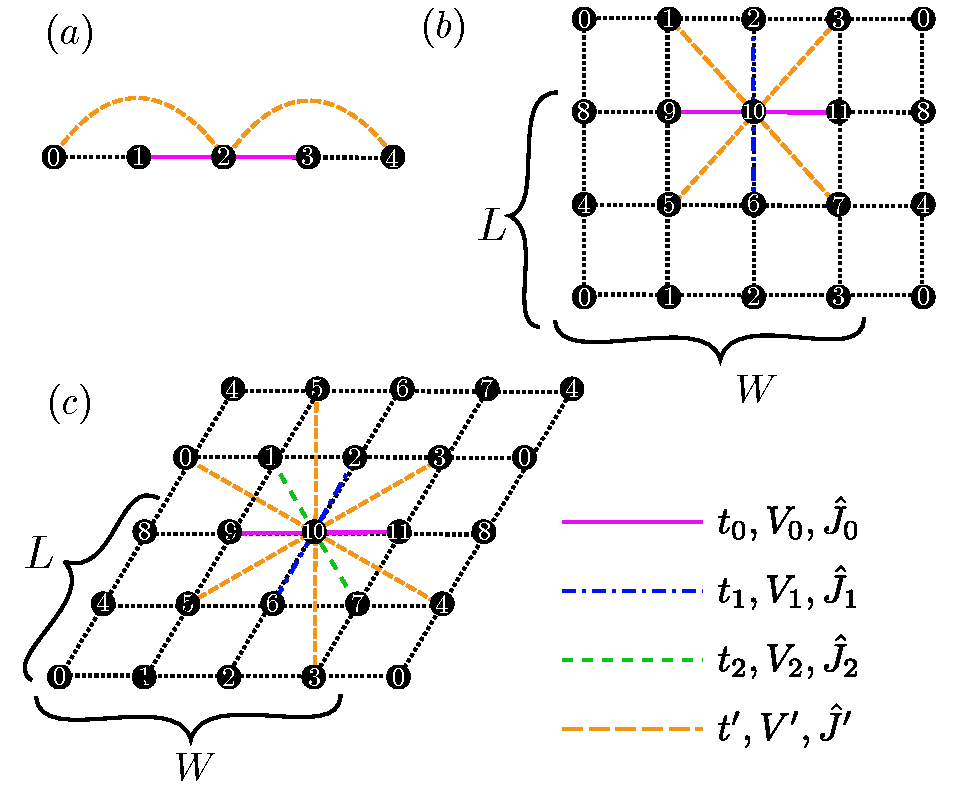
\includegraphics[width=10cm]{../figs/chap04_1_lattice.pdf}
    \caption{(a)1次元鎖、(b)2次元正方格子、(c)2次元三角格子の模式図. 
      ホッピング積分、オフサイトクーロン積分、スピン結合は、
      再近接サイト間(マゼンタの実線)ではそれぞれ$t,V,J$となり、
      次近接サイト間(緑の破線)ではそれぞれ$t',V',J'$となります。}
    \label{fig_chap04_1_lattice}
  \end{center}
\end{figure}

\begin{figure}[!htbp]
  \begin{center}
    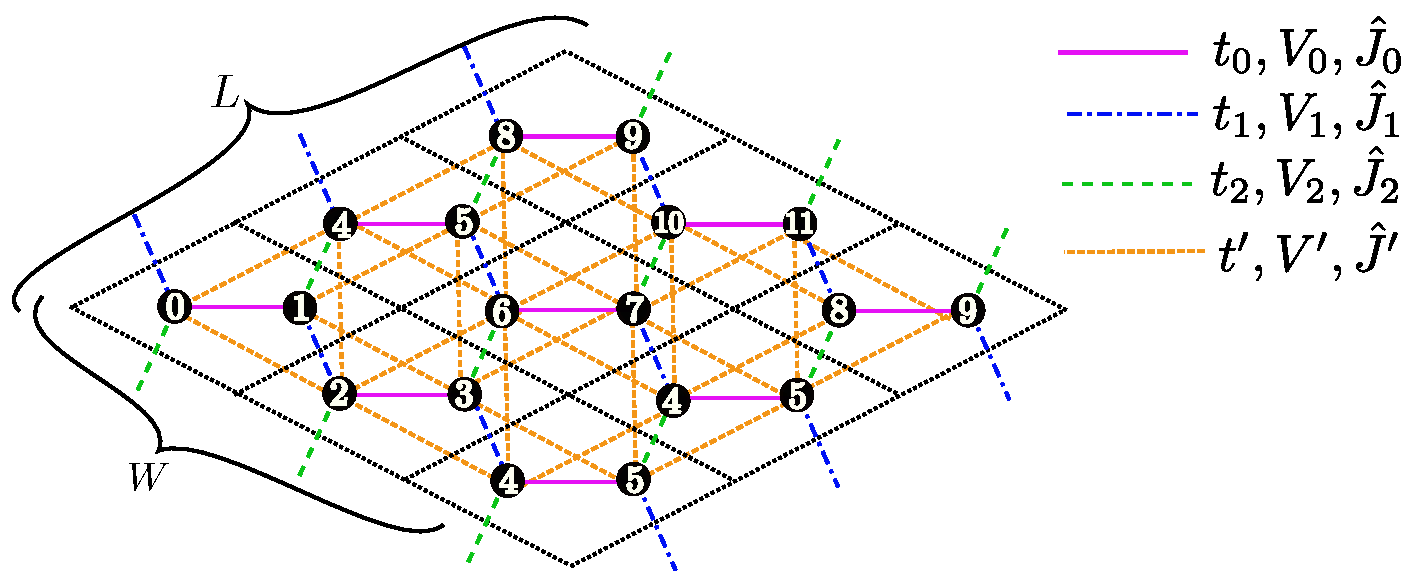
\includegraphics[width=15cm]{../figs/chap04_1_honeycomb.pdf}
    \caption{2次元異方的蜂の巣格子の模式図. 
      ホッピング積分、オフサイトクーロン積分、スピン結合は、
      ボンドの方向によって異なります。
      また、次近接のホッピング積分、オフサイトクーロン積分、スピン結合
      には対応していません。
    }
    \label{fig_chap04_1_honeycomb}
  \end{center}
\end{figure}

\begin{figure}[!htbp]
  \begin{center}
    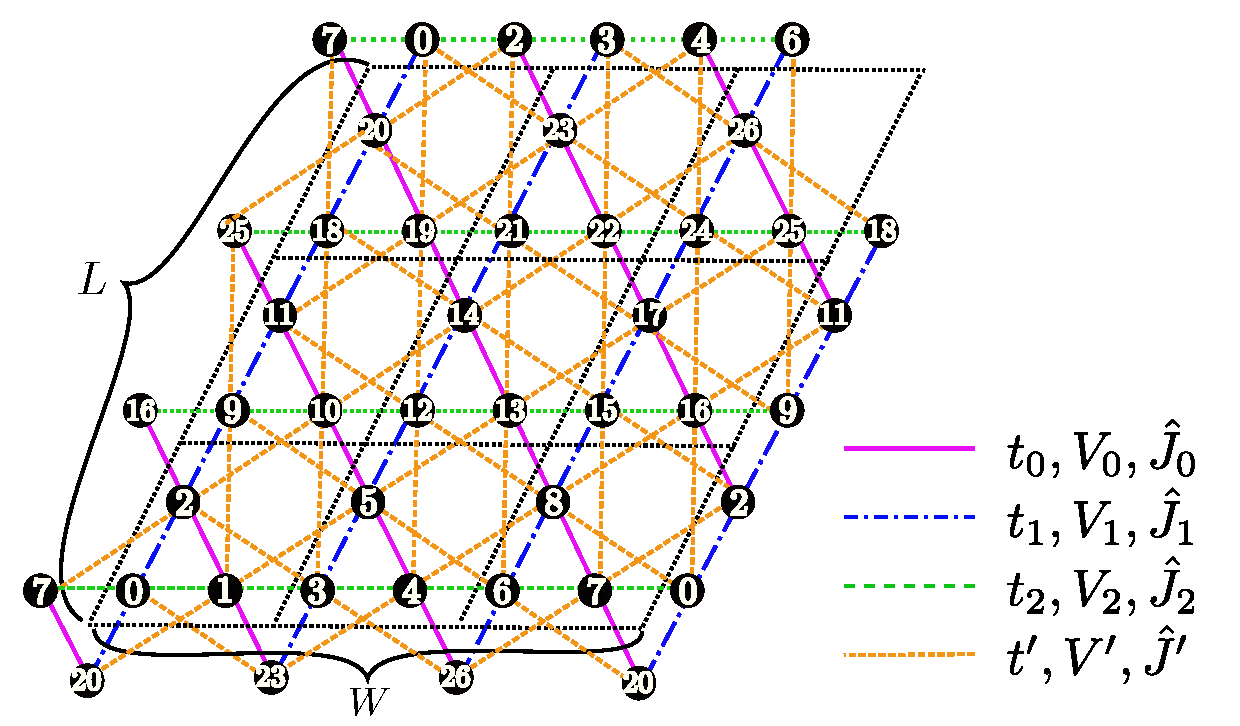
\includegraphics[width=15cm]{../figs/kagome.pdf}
    \caption{カゴメ格子の模式図. 
    }
    \label{fig_kagome}
  \end{center}
\end{figure}

\begin{figure}[!htbp]
  \begin{center}
    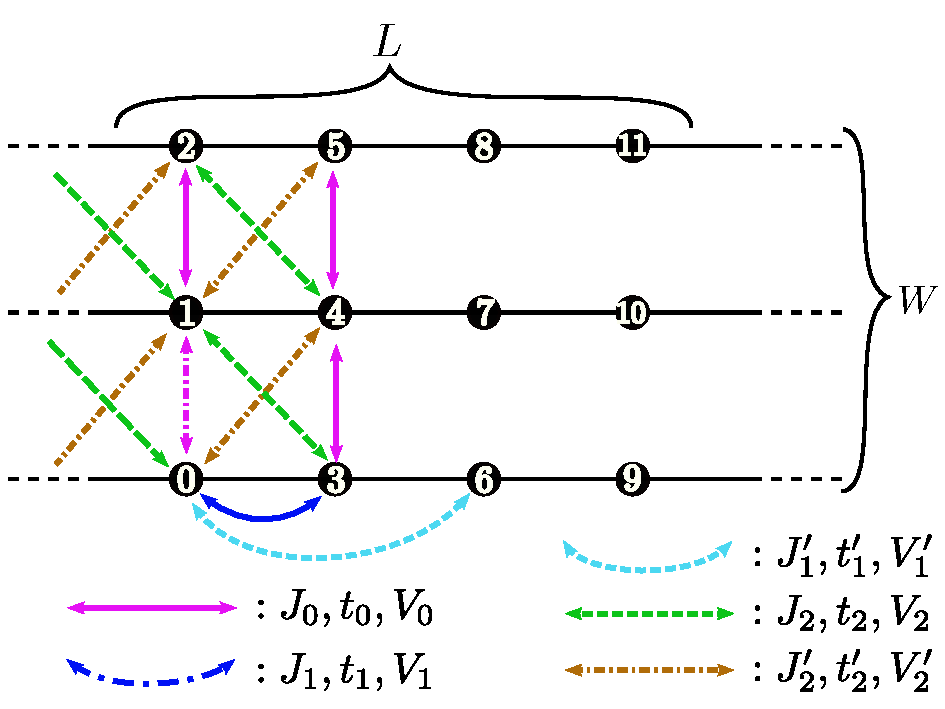
\includegraphics[width=10cm]{../figs/ladder.pdf}
    \caption{梯子格子の模式図. 
    }
    \label{fig_ladder}
  \end{center}
\end{figure}

\end{itemize}

\subsection{格子に関するパラメーター}

\subsubsection{1次元鎖[Fig. \ref{fig_chap04_1_lattice}(a)]}

\begin{itemize}

\item \verb|L|

{\bf 形式 :} 自然数

{\bf 説明 :} 鎖の長さを指定します. 

\end{itemize}

\subsubsection{梯子格子(Fig. \ref{fig_ladder})}

\begin{itemize}

\item \verb|L|

{\bf 形式 :} 自然数

{\bf 説明 :} 梯子の長さを指定します. 

\item \verb|W|

{\bf 形式 :} 自然数

{\bf 説明 :} 梯子の本数を指定します. 

\end{itemize}

\begin{figure}[!htbp]
  \begin{center}
    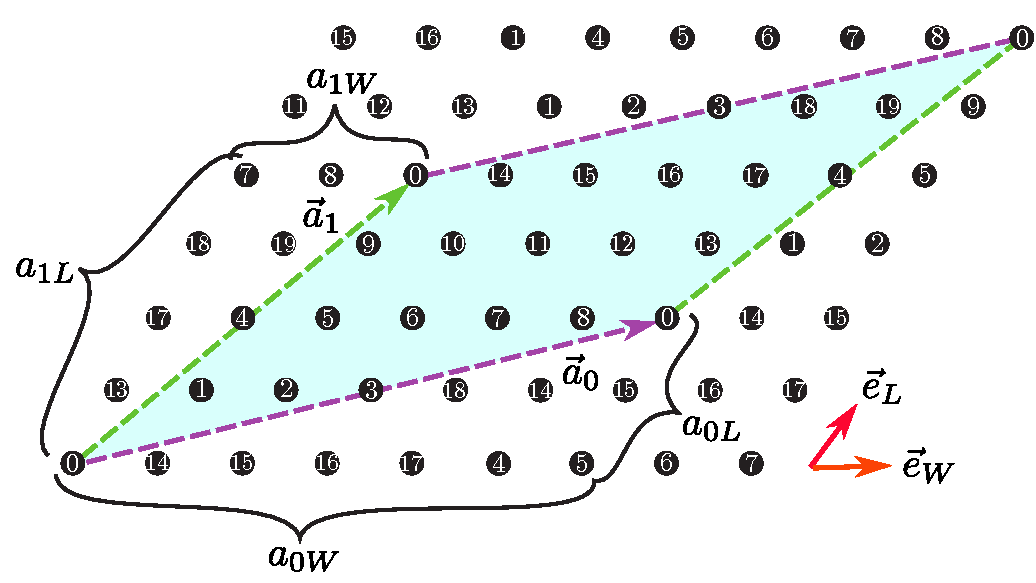
\includegraphics[width=15cm]{../figs/chap04_1_unitlattice.pdf}
    \caption{三角格子において、${\vec a}_0 = (6, 2), {\vec a}_1 = (2, 4)$とした場合のセル形状。
      ${\vec a}_0$(マゼンタ)および${\vec a}_1$(グリーン)
      で囲まれた部分(サイト数は20)が計算するセルとなる。
    }
    \label{fig_chap04_1_unitlattice}
  \end{center}
\end{figure}

\subsubsection{矩形格子[Fig. \ref{fig_chap04_1_lattice}(b)]、 
三角格子[Fig. \ref{fig_chap04_1_lattice}(c)]、
蜂の巣格子(Fig. \ref{fig_chap04_1_honeycomb})、
カゴメ格子(Fig. \ref{fig_kagome})}

これらの格子では、標準の単位胞(図中の黒の破線を参照)を用いて格子形状を指定する方法と、
それらとは別の方向に格子ベクトルを取る方法が選択できます。
また、両方を指定した場合にはプログラムを終了します。

\begin{itemize}

\item \verb|W|, \verb|L|

{\bf 形式 :} 自然数

{\bf 説明 :} 標準の単位胞の並び方を指定します。

\item \verb|a0W|, \verb|a0L|, \verb|a1W|, \verb|a1L|

{\bf 形式 :} 自然数

{\bf 説明 :} 格子を指定する2本のベクトル(${\vec a}_0, {\vec a}_1$)
を指定します (Fig. \ref{fig_chap04_1_unitlattice})。
これらのベクトルは標準の並進ベクトルを基底とした座標(Fractional coordinate)
で指定されます。

\end{itemize}

スタンダードモードで出力される\verb|lattice.gp|というファイルを使うと、
自分の意図した通りの格子のとり方になっているかどうかを確かめる事が出来ます。
このファイルは、次のようにして\verb|gnuplot|に読み込ませることが出来ます。
\begin{verbatim}
$ gnuplot lattice.gp
\end{verbatim}

\subsection{副格子}

以下パラメータを用いると変分波動関数のペア軌道部分に副格子の周期性を持たせることが出来ます。

\begin{itemize}

\item \verb|a0Wsub|, \verb|a0Lsub|, \verb|a1Wsub|, \verb|a1Lsub|, \verb|Wsub|, \verb|Lsub|

{\bf 形式 :} 自然数。デフォルトでは
\verb|a0Wsub=a0W|, \verb|a0Lsub=a0L|, \verb|a1Wsub=a1W|, \verb|a1Lsub=a1L|, 
\verb|Wsub=W|, \verb|Lsub=L|となる。

{\bf 説明 :} これらのパラメーターの指定の仕方は
\verb|a0W|, \verb|a0L|, \verb|a1W|, \verb|a1L|, \verb|W|, \verb|L|
と同様です。
ただし、元の計算セルが副格子に整合しない場合にはプログラムを終了します。

\end{itemize}

%\subsection{保存量に関するパラメーター}
%
%\begin{itemize}
%\item \verb|nelec|
%
%{\bf 形式 :} 整数
%
%{\bf 説明 :} 全伝導電子数を指定します。
%\verb|model = "Fermion HubbardGC"|, \verb|"Spin"|, \verb|"SpinGC"|
%のときには指定しないでください。

%\item \verb|2Sz|

%{\bf 形式 :} 整数

%{\bf 説明 :} 全スピンのz 成分の2倍を指定します。
%\verb|model = "Fermion HubbardGC"|, \verb|SpinGC|
%のときには指定しないでください。
%\end{itemize}

\subsection{ハミルトニアンの各項の係数}

デフォルト値は特に記載されていないものについては0に設定してあります。
型が複素数のパラメータは「実部, 虚部」(間に``,'')の形式で指定し、
実数の場合には「実部」で指定が可能です。

\subsubsection{局所項}

\begin{itemize}

\item \verb|mu|

{\bf 形式 :} 実数

{\bf 説明 :} Hubbardおよび近藤格子模型での化学ポテンシャルを指定します。

\item \verb|U|

{\bf 形式 :} 実数

{\bf 説明 :} Hubbardおよび近藤格子模型でのオンサイトクーロン積分を指定します。

\item \verb|Jx|, \verb|Jy|, \verb|Jz|, \verb|Jxy|, 
  \verb|Jyx|, \verb|Jxz|, \verb|Jzx|, \verb|Jyz|, \verb|Jzy|

{\bf 形式 :} 実数

{\bf 説明 :} 近藤格子模型での、局在電子と遍歴電子のスピン結合を指定します。
また対角項について, \verb|Jx, Jy, Jz|を指定する代わりに、パラメータ\verb|J|を指定すると
\verb|Jx = Jy = Jz = J|が代入されます。
\verb|J|を指定した上で\verb|Jx|, \verb|Jy|, \verb|Jz|を指定した場合はプログラムを終了します。

\item \verb|h|, \verb|Gamma|, \verb|D|

{\bf 形式 :} 実数

{\bf 説明 :} スピン模型での縦磁場、横磁場、異方性パラメータを指定します。

\end{itemize}

下記の非局所項は、梯子格子の場合とそれ以外(1次元鎖、矩形格子、三角格子、蜂の巣格子、カゴメ格子)
の場合で指定の仕方が異なります。
また、各格子で指定可能なパラメーターをTable \ref{table_interactions}に表します。

\begin{table}[hbp]
  \begin{tabular}{|l||c|c|c|c|c|c|c|c|} \hline
    相互作用 & 1次元鎖 & 矩形格子 & 三角格子 & 蜂の巣格子 & カゴメ格子 & 梯子格子\\ 
    \hline \hline
     \verb|J|, \verb|t|, \verb|V|(省略形) & $\circ$	 & $\circ$ & $\circ$ & $\circ$ & $\circ$ & -\\ 
     \hline
    \verb|J'|, \verb|t'|, \verb|V'| & $\circ$	 & $\circ$	& $\circ$ 	& $\circ$ 	& $\circ$ & - \\ 
    \hline
    \verb|J0|, \verb|t0|, \verb|V0| & $\circ$  & $\circ$ 	& $\circ$ 	& $\circ$ 	& $\circ$ & $\circ$\\ 
    \hline
    \verb|J1|, \verb|t1|, \verb|V1| & -         	 & $\circ$ 	& $\circ$ 	& $\circ$ 	& $\circ$ & $\circ$\\ 
    \hline
    \verb|J2|, \verb|t2|, \verb|V2|  & -         	 & -    	& $\circ$ 	& $\circ$ 	& $\circ$ & $\circ$\\
    \hline
    \verb|J1'|, \verb|t1'|, \verb|V1'| & -		 &-	 	& -		& -		& -		& $\circ$\\
    \hline
    \verb|J2'| ,\verb|t2'|, \verb|V2'|  & -		 &-	 	& -		& -		& -		& $\circ$\\ 
    \hline
\end{tabular}
   \caption{各格子で定義可能な相互作用一覧。ただし、スピン結合については行列として与えることが可能。}
    \label{table_interactions}
\end{table}

\subsubsection{非局所項[梯子格子 (Fig. \ref{fig_ladder})]}

\begin{itemize}
\item \verb|t0|,  \verb|t1|,  \verb|t1'|,  \verb|t2|,  \verb|t2'|

{\bf 形式 :} 複素数

{\bf 説明 :} 梯子格子でのホッピング(Fig. \ref{fig_ladder}参照)を指定します。

\item \verb|V0|,  \verb|V1|,  \verb|V1'|,  \verb|V2|,  \verb|V2'|

{\bf 形式 :} 実数

{\bf 説明 :} 梯子格子でのオフサイトクーロン積分
(Fig. \ref{fig_ladder}参照)を指定します。

\item \verb|J0x|, \verb|J0y|, \verb|J0z|, \verb|J0xy|, 
  \verb|J0yx|, \verb|J0xz|, \verb|J0zx|, \verb|J0yz|, \verb|J0zy|
\item \verb|J1x|, \verb|J1y|, \verb|J1z|, \verb|J1xy|, 
  \verb|J1yx|, \verb|J1xz|, \verb|J1zx|, \verb|J1yz|, \verb|J1zy|
\item \verb|J1'x|, \verb|J1'y|, \verb|J1'z|, \verb|J1'xy|, 
  \verb|J1'yx|, \verb|J1'xz|, \verb|J1'zx|, \verb|J1'yz|, \verb|J1'zy|
\item \verb|J2x|, \verb|J2y|, \verb|J2z|, \verb|J2xy|, 
  \verb|J2yx|, \verb|J2xz|, \verb|J2zx|, \verb|J2yz|, \verb|J2zy|
\item \verb|J2'x|, \verb|J2'y|, \verb|J2'z|, \verb|J2'xy|, 
  \verb|J2'yx|, \verb|J2'xz|, \verb|J2'zx|, \verb|J2'yz|, \verb|J2'zy|

{\bf 形式 :} 実数

{\bf 説明 :} 梯子格子でのスピン相互作用
(Fig. \ref{fig_ladder}参照)を指定します。
また対角項について、例えば\verb|J0x, J0y, J0z|を指定する代わりに
パラメータ\verb|J0|を指定すると
\verb|J0x = J0y = J0z = J0|が代入されます。
\verb|J0|を指定した上で\verb|J0x, J0y, J0z|等も指定した場合はプログラムを終了します。
\verb|J1|, \verb|J1'|, \verb|J2|, \verb|J2'|についても同様です。

\end{itemize}

\subsubsection{非局所項 [梯子格子以外(Figs. \ref{fig_chap04_1_lattice}, \ref{fig_chap04_1_honeycomb},
\ref{fig_kagome})]}

\begin{itemize}
\item \verb|t0|,  \verb|t1|, \verb|t2|

{\bf 形式 :} 複素数

{\bf 説明 :} Hubbardおよび近藤格子模型での、最近接サイト間の各方向のホッピングを指定します。
また、ホッピングのボンド方向依存性がない場合は\verb|t0|,  \verb|t1|, \verb|t2|を
別々に指定する代わりにパラメータ\verb|t|を指定すると、\verb|t0 = t1 = t2 = t|が代入されます。
\verb|t|と\verb|t0|等の両方が指定された場合にはプログラムを終了します。

\item \verb|V0|,  \verb|V1|, \verb|V2|

{\bf 形式 :} 実数

{\bf 説明 :} Hubbardおよび近藤格子模型での、最近接サイト間のCoulomb積分を指定します。
また、サイト間Coulomb積分のボンド方向依存性がない場合は\verb|V0|,  \verb|V1|, \verb|V2|を
別々に指定する代わりにパラメータ\verb|V|を指定すると、\verb|V0 = V1 = V2 = V|が代入されます。
\verb|V|と\verb|V0|等の両方が指定された場合にはプログラムを終了します。

\item \verb|J0x|, \verb|J0y|, \verb|J0z|, \verb|J0xy|, 
  \verb|J0yx|, \verb|J0xz|, \verb|J0zx|, \verb|J0yz|, \verb|J0zy|
\item \verb|J1x|, \verb|J1y|, \verb|J1z|, \verb|J1xy|, 
  \verb|J1yx|, \verb|J1xz|, \verb|J1zx|, \verb|J1yz|, \verb|J1zy|
\item \verb|J2x|, \verb|J2y|, \verb|J2z|, \verb|J2xy|, 
  \verb|J2yx|, \verb|J2xz|, \verb|J2zx|, \verb|J2yz|, \verb|J2zy|

{\bf 形式 :} 実数

{\bf 説明 :} スピン模型での、最近接サイト間のスピン相互作用を指定します。
また対角項について、例えば\verb|J0x, J0y, J0z|を指定する代わりに
パラメータ\verb|J0|を指定すると
\verb|J0x = J0y = J0z = J0|が代入されます。
\verb|J0|を指定した上で\verb|J0x, J0y, J0z|等も指定した場合はプログラムを終了します。
\verb|J1|, \verb|J2|についても同様です。

スピン間相互作用のボンド方向依存性がない場合には、
\verb|Jx|, \verb|Jy|, \verb|Jz|, \verb|Jxy|, 
\verb|Jyx|, \verb|Jxz|, \verb|Jzx|, \verb|Jyz|, \verb|Jzy|
を指定すると、\verb|J0x = J1x = J2x = Jx|のようにすべてのボンド方向のスピン間相互作用に
同じ値を代入することが出来ます。
\verb|Jx|$\sim$\verb|Jzy|系列のどれかと\verb|J0x|$\sim$\verb|J2zy|系列のどれかを両方指定した
場合にはプログラムを終了します。
以下に最近接間スピン相互作用の指定方法の例を挙げます。

\begin{itemize}

\item ボンド方向依存性、スピン方向依存性、相互作用の非対角成分($J_{x y}$等)がない場合

\verb|J|を指定

\item ボンド方向依存性、相互作用の非対角成分がなく、スピン方向依存性がある場合

\verb|Jx, Jy, Jz|のうち\verb|0|でないものを指定

\item ボンド方向依存性がなく、スピン方向依存性、相互作用の非対角成分がある場合

\verb|Jx, Jy, Jz, Jxy, Jyz, Jxz, Jyx, Jzy, Jzx|のうち\verb|0|でないものを指定

\item スピン方向依存性、相互作用の非対角成分がなく、ボンド方向依存性がある場合

\verb|J0, J1, J2|のうち\verb|0|でないものを指定

\item スピン方向依存性がなく、ボンド方向依存性、相互作用の非対角成分がある場合

\verb|J0x, J0y, J0z, J1x, J1y, J1z, J2x, J2y, J2z|のうち\verb|0|でないものを指定

\item ボンド方向依存性、スピン方向依存性、相互作用の非対角成分がある場合

\verb|J0x|$\sim$\verb|J2zy|のすべてのうち\verb|0|でないものを指定

\end{itemize}
\item \verb|t'|

{\bf 形式 :} 複素数

{\bf 説明 :} Hubbardおよび近藤格子模型での、次近接サイト間の各方向のホッピングを指定します。

\item \verb|V'|

{\bf 形式 :} 実数

{\bf 説明 :} Hubbardおよび近藤格子模型での、次近接サイト間のCoulomb積分を指定します。

\item \verb|J'x|, \verb|J'y|, \verb|J'z|, \verb|J'xy|, 
  \verb|J'yx|, \verb|J'xz|, \verb|J'zx|, \verb|J'yz|, \verb|J'zy|

{\bf 形式 :} 実数

{\bf 説明 :} スピン模型での、次近接サイト間のスピン相互作用を指定します。
また対角項について、\verb|J'x, J'y, J'z|を指定する代わりに
パラメータ\verb|J'|を指定すると
\verb|J'x = J'y = J'z = J'|が代入されます。
\verb|J'|を指定した上で\verb|J'x, J'y, J'z|も指定した場合はプログラムを終了します。

\item \verb|phase0|, \verb|phase1|

  {\bf 形式 :} 複素数(デフォルトでは\verb|1.0|)
  
  {\bf 説明 :} 計算するセルの境界をまたいだホッピング項に付く位相因子を指定することが出来ます。
  $\vec{a}_0$方向、$\vec{a}_1$方向それぞれ別の位相因子を用いることが出来ます。
  1次元系では\verb|phase0|のみ使用できます。
  例えば、$i$サイトから$i+1$サイトへのホッピングで、
  正の方向に境界をまたいだ場合には次のようになります。
  \begin{align}
    ({\rm phase0}) \times t {\hat c}_{i+1 \sigma}^\dagger {\hat c}_{i \sigma}
    + ({\rm phase0})^* \times t^* {\hat c}_{i \sigma}^\dagger {\hat c}_{i+1 \sigma}
  \end{align}

\end{itemize}

\subsection{計算条件のパラメーター}

\begin{itemize}

\item \verb|OutputMode|

  {\bf 形式 :} \verb|"none"|, \verb|"correlation"|, \verb|"full"|のいずれか(デフォルトは\verb|correlation|)

  {\bf 説明 :} 計算を行う相関関数を指定します。
\verb|"none"|の場合は相関関数を計算しません。
\verb|"correlation"|を指定した場合には、1体部分はすべての$i, \sigma$について
$\langle c_{i \sigma}^{\dagger}c_{i \sigma} \rangle$を、
2体部分はすべての$i, j, \sigma, \sigma'$について
$\langle c_{i \sigma}^{\dagger}c_{i \sigma} c_{j \sigma'}^{\dagger}c_{j \sigma'} \rangle$
を計算します。
\verb|"full"|を指定した場合には、
1体部分はすべての$i, j, \sigma, \sigma'$について
$\langle c_{i \sigma}^{\dagger}c_{j \sigma'} \rangle$を、
2体部分はすべての$i_1, i_2, i_3, i_4, \sigma_1, \sigma_2, \sigma_3, \sigma_4$について
$\langle c_{i_1 \sigma_1}^{\dagger}c_{i_2 \sigma_2} c_{i_3 \sigma_3}^{\dagger}c_{i_4 \sigma_4} \rangle$
を計算します。
スピン系の演算子はBogoliubov表現により生成消滅演算子で表されています。
詳しくは\ref{sec_bogoliubov_rep}をご覧ください。

  \item  \verb|CDataFileHead|

 {\bf 形式 :} string型 (空白不可、必須)

{\bf 説明 :} アウトプットファイルのヘッダ。例えば、一体のGreen関数の出力ファイル名が{\bf xxx\_cisajs.dat}として出力されます(xxxに\verb|CDataFileHead|で指定した文字が記載)。

 \item  \verb|CParaFileHead|

 {\bf 形式 :} string型 (空白不可、必須)

{\bf 説明 :} 最適化された変分パラメータの出力ファイル名のヘッダ。最適化された変分パラメータが{\bf xxx\_opt.dat}ファイルとして出力されます(xxxに\verb|CParaFileHead|で指定した文字が記載)。
 
 
 \item  \verb|NVMCCalMode|

 {\bf 形式 :} int型 (\tr{デフォルト値 = 0})

{\bf 説明 :} [0] 変分パラメータの最適化、[1] 1 体・2 体のグリーン関数の計算。
 
 \item  \verb|NLanczosMode|

 {\bf 形式 :} int型 (\tr{デフォルト値 = 0})

{\bf 説明 :} [0] 何もしない、[1] Single Lanczos Step でエネルギーまで計算、
[2] Single Lanczos Step で1 体・2 体のグリーン関数まで計算
(条件: 1, 2 は\verb|NVMCCalMode| = 1のみ使用可能. 
また, pair hopping項, exchange 項がハミルトニアンに含まれる場合は使用できません)。
 
 \item  \verb|NDataIdxStart|

 {\bf 形式 :} int型 (\tr{デフォルト値 = 1})

{\bf 説明 :} 出力ファイルの付加番号。
\verb|NVMCCalMode|= 0 の場合は\verb|NDataIdxStart|が出力され、 
\verb|NVMCCalMode| = 1 の場合は、
\verb|NDataIdxStart|から連番で\verb|NDataQtySmp|個のファイルを出力します。
   
 \item  \verb|NDataQtySmp|

 {\bf 形式 :} int型 (\tr{デフォルト値 = 1})

{\bf 説明 :} 出力ファイルのセット数。 \verb|NVMCCalMode| = 1 の場合に使用します。

\item  \verb|nelec|

  {\bf 形式 :} {int型 (1以上、必須)}

  {\bf 説明 :} \tr{伝導電子の数。
    $\uparrow$電子と$\downarrow$電子の個数を足したものを入力してください。}

\item  \verb|NSPGaussLeg|

  {\bf 形式 :} {int型 (1以上、\tr{デフォルト値 = 8})}

  {\bf 説明 :} スピン量子数射影の$\beta$積分($S^y$回転)のGauss-Legendre求積法の分点数。


\item  \verb|NSPStot|

  {\bf 形式 :} int型 (0以上、\tr{デフォルト値 = 0})

  {\bf 説明 :}  スピン量子数。

\item  \verb|NMPTrans|

  {\bf 形式 :} int型 (1以上、\tr{デフォルト値は副格子内部の並進ベクトルの数})

  {\bf 説明 :} 
  運動量・格子対称性の量子数射影の個数。
  TransSymファイルで指定した重みで上から\verb|NMPTrans|個まで使用する。\tr{射影を行わない場合は1に設定する。}

 \item  \verb|NSROptItrStep|

{\bf 形式 :} int型 (1以上、\tr{デフォルト値 = 1000})

{\bf 説明 :} 
SR 法で最適化する場合の全ステップ数。\verb|NVMCCalMode|=0の場合のみ使用されます。
 
 \item  \verb|NSROptItrSmp|

{\bf 形式 :} int型 (1以上数、\tr{デフォルト値 = }\verb|NSROptItrStep|/10)

{\bf 説明 :} \verb|NSROptItrStep|ステップ中、最後の\verb|NSROptItrSmp|ステップでの各変分パラメータの平均値を最適値とする。\verb|NVMCCalMode|=0の場合のみ使用されます。

\item   \verb|DSROptRedCut|
   
{\bf 形式 :} double型 (\tr{デフォルト値 = 0.001})

{\bf 説明 :} SR 法安定化因子。手法論文の$\varepsilon_{\rm wf}$に対応。

 \item  \verb|DSROptStaDel| 
   
 {\bf 形式 :} double型 (\tr{デフォルト値 = 0.02})

  {\bf 説明 :} SR 法安定化因子。手法論文の$\varepsilon$に対応。
     
\item \verb|DSROptStepDt|

{\bf 形式 :} double型 (\tr{デフォルト値 = 0.02})

{\bf 説明 :} \tr{要確認(マニュアルに説明なし)}
 
\item \verb|NVMCWarmUp|

{\bf 形式 :} int型 (1以上、\tr{デフォルト値=10})

{\bf 説明 :}マルコフ連鎖の空回し回数。

\item \verb|NVMCIniterval|

{\bf 形式 :} int型 (1以上、\tr{デフォルト値=1})

{\bf 説明 :} サンプル間のステップ間隔。ローカル更新が\verb|Nsite|× \verb|NVMCIniterval| 回行わます。

\item \verb|NVMCSample|

{\bf 形式 :} int型 (1以上、\tr{デフォルト値=1000})

{\bf 説明 :} 期待値計算に使用するサンプル数。

\item \verb|RndSeed|

{\bf 形式 :} int型 

{\bf 説明 :} 乱数の初期seed。\tr{MPI 並列では各計算機に}\verb|RndSeed|\tr{+my rank+1 で初期seed が与えられます。}

 \item \verb|NSplitSize|

{\bf 形式 :} int型 (1以上、\tr{デフォルト値=1})

{\bf 説明 :} mpi内部並列を行う場合の並列数。

\item \verb|NStoreOO|

{\bf 形式 :} int型 (1以上、\tr{デフォルト値=0})

{\bf 説明 :} 期待値$\langle O_k O_l \rangle$を計算するとき行列-行列積にするオプション(1で機能On)。
 
\item  \verb|ComplexType|
  
  {\bf 形式 :} int型 (\verb|0|もしくは\verb|1|、デフォルト値\verb|0|)

  {\bf 説明 :} \verb|0|のとき変分パラメータの実部のみを、\verb|1|のとき実部/虚部両方を最適化します。

\end{itemize}


\newpage
\section{詳細入力ファイル}
\label{Ch:HowToExpert}

mVMCで使用する詳細入力ファイル(*def)に関して説明します。
入力ファイルの種別は以下の6つで分類されます。
\begin{description}
\item[(1)~List:]
~\\{キーワード指定なし}:
使用するinput fileの名前のリストを書きます。なお、ファイル名は任意に指定することができます。
\item[(2)~Basic parameters:]
~\\{\bf ModPara}: 計算時に必要な基本的なパラメーター(サイトの数、電子数など)を設定します。
~\\{\bf LocSpin}: 局在スピンの位置を設定します。
\item[(3)~Set Hamiltonian:] 
~\\以下のファイルを用い、Hamiltonianを電子系の表式により指定します。
~\\{\bf Trans}: $c_{i\sigma_1}^{\dag}c_{j\sigma_2}$で表される一体項を指定します。
~\\{\bf InterAll}: $c_ {i \sigma_1}^{\dag}c_{j\sigma_2}c_{k \sigma_3}^{\dag}c_{l \sigma_4}$で表される一般二体相互作用を指定します。\\
~\\なお、使用頻度の高い相互作用に関しては下記のキーワードで指定することも可能です。
~\\{\bf CoulombIntra}: $n_ {i \uparrow}n_{i \downarrow}$で表される相互作用を指定します($n_{i \sigma}=c_{i\sigma}^{\dag}c_{i\sigma}$)。
~\\{\bf CoulombInter}: $n_ {i}n_{j}$で表される相互作用を指定します($n_i=n_{i\uparrow}+n_{i\downarrow}$)。
~\\{\bf Hund}: $n_{i\uparrow}n_{j\uparrow}+n_{i\downarrow}n_{j\downarrow}$で表される相互作用を指定します。
~\\{\bf PairHop}:  $c_ {i \uparrow}^{\dag}c_{j\uparrow}c_{i \downarrow}^{\dag}c_{j  \downarrow}$で表される相互作用を指定します。
~\\{\bf Exchange}: $S_i^+ S_j^-$で表される相互作用を指定します。
\item[(4)~Set condition of variational parameters :] 
~\\変分波動関数は
\begin{equation}
|\psi \rangle = {\cal P}_G{\cal P}_J{\cal P}_{d-h}^{(2)}{\cal P}_{d-h}^{(4)}{\cal L}^S{\cal L}^K{\cal L}^P |\phi_{\rm pair} \rangle,
\end{equation}
で与えられます。ここで、一体部分は実空間のペア関数
\begin{equation}
|\phi_{\rm pair} \rangle = \left[\sum_{i, j=1}^{N_s} f_{ij}c_{i\uparrow}^{\dag}c_{j\downarrow}^{\dag} \right]^{N/2}|0 \rangle,
\end{equation}
を用いた波動関数で表されます。ここで$N$は全電子数、$N_s$は全サイト数です。
変分パラメータを最適化するかどうかについては以下のファイルを用いて指定します。
~\\{\bf Gutzwiller}: ${\cal P}_G=\exp\left[ \sum_i g_i n_{i\uparrow} n_{i\downarrow} \right]$のうち、最適化の対象とする変分パラメータ$g_i$を指定します。
~\\{\bf Jastrow}: ${\cal P}_J=\exp\left[\frac{1}{2} \sum_{i\neq j} v_{ij} n_i n_j\right]$のうち、最適化の対象とする変分パラメータ$v_{ij}$を指定します。
~\\{\bf DH2}:  ${\cal P}_{d-h}^{(2)}= \exp \left[ \sum_t \sum_{n=0}^2 (\alpha_{2nt}^d \sum_{i}\xi_{i2nt}^d+\alpha_{2nt}^h \sum_{i}\xi_{i2nt}^h)\right]$で表される2サイトのdoublon-holon相関因子を指定します。詳細はDH2ファイルの説明を参照してください。
~\\{\bf DH4}:  ${\cal P}_{d-h}^{(4)}= \exp \left[ \sum_t \sum_{n=0}^4 (\alpha_{4nt}^d \sum_{i}\xi_{i4nt}^d+\alpha_{4nt}^h \sum_{i}\xi_{i4nt}^h)\right]$で表される4サイトのdoublon-holon相関因子を指定します。詳細はDH4ファイルの説明を参照してください。
~\\{\bf Orbital}: ペア軌道$|\phi_{\rm pair} \rangle = \left[\sum_{i, j=1}^{N_s} f_{ij}c_{i\uparrow}^{\dag}c_{j\downarrow}^{\dag} \right]^{N/2}|0 \rangle$を設定します。
~\\{\bf TransSym}: 運動量射影${\cal L}_K=\frac{1}{N_s}\sum_{{\bm R}}e^{i {\bm K} \cdot{\bm R} } \hat{T}_{\bm R}$と格子対称性射影${\cal L}_P=\sum_{\alpha}p_{\alpha} \hat{G}_{\alpha}$に関する指定を行います。ここで、${\bm K}$は全運動量、$\hat{T}_{\bm R}$は並進ベクトル${\bm R}$に対応する並進演算子、$\hat{G}_{\alpha}$は格子の点群演算子、$p_\alpha$はパリティをそれぞれ表します。

\item[(5)~Initial variational parameters:]
~\\ 変分パラメータに関する初期値を与えます。キーワード指定されない場合には$0$が初期値として設定されます。
~\\{\bf InGutzwiller}: ${\cal P}_G=\exp\left[ \sum_i g_i n_{i\uparrow} n_{i\downarrow} \right]$のうち、変分パラメータ$g_i$の初期値を指定します。
~\\{\bf InJastrow}: ${\cal P}_J=\exp\left[\frac{1}{2} \sum_{i\neq j} v_{ij} n_i n_j\right]$のうち、変分パラメータ$v_{ij}$の初期値を指定します。
~\\{\bf InDH2}:  ${\cal P}_{d-h}^{(2)}= \exp \left[ \sum_t \sum_{n=0}^2 (\alpha_{2nt}^d \sum_{i}\xi_{i2nt}^d+\alpha_{2nt}^h \sum_{i}\xi_{i2nt}^h)\right]$で表される2サイトのdoublon-holon相関因子$\alpha_{2nt}^{d(h)}$の初期値を指定します。
~\\{\bf InDH4}:  ${\cal P}_{d-h}^{(4)}= \exp \left[ \sum_t \sum_{n=0}^4 (\alpha_{4nt}^d \sum_{i}\xi_{i4nt}^d+\alpha_{4nt}^h \sum_{i}\xi_{i4nt}^h)\right]$で表される4サイトのdoublon-holon相関因子$\alpha_{4nt}^{d(h)}$の初期値を指定します。
~\\{\bf InOrbital}: ペア軌道$|\phi_{\rm pair} \rangle = \left[\sum_{i, j=1}^{N_s} f_{ij}c_{i\uparrow}^{\dag}c_{j\downarrow}^{\dag} \right]^{N/2}|0 \rangle$の$ f_{ij}$に関する初期値を設定します。


\item[(6)~Output:]
~\\{\bf OneBodyG }:出力する一体Green関数を指定します。
 $\langle c^{\dagger}_{i\sigma_1}c_{j\sigma_2}\rangle$が出力されます。

 {\bf TwoBodyG }:出力する二体Green関数を指定します。
 $\langle c^{\dagger}_{i\sigma_1}c_{j\sigma_2}c^{\dagger}_{k \sigma_3}c_{l\sigma_4}\rangle$
が出力されます。
\end{description}
%%%%%%%%%%%%%%%%%%%%%%
\newpage
~\subsection{入力ファイル指定用ファイル}
\label{Subsec:InputFileList}
計算で使用する入力ファイル一式を指定します。ファイル形式に関しては、以下のようなフォーマットをしています。\\
\begin{minipage}{10cm}
\begin{screen}
\begin{verbatim}
ModPara  modpara.def
LocSpin  zlocspn.def
Trans    ztransfer.def
InterAll zinterall.def
Orbital orbitalidx.def
OneBodyG zcisajs.def
TwoBodyG	zcisajscktaltdc.def
\end{verbatim}
\end{screen}
\end{minipage}
\\
\subsubsection{ファイル形式}
[string01]~[string02]
\subsubsection{パラメータ}
 \begin{itemize}
   \item  $[$string01$]$
   
   {\bf 形式 :} string型 (固定)
   
   {\bf 説明 :} キーワードを指定します。
   
   \item  $[$string02$]$
   
    {\bf 形式 :} string型 

   {\bf 説明 :} キーワードにひも付けられるファイル名を指定します(任意)。
 \end{itemize}
\subsubsection{使用ルール}
本ファイルを使用するにあたってのルールは以下の通りです。
\begin{itemize}
\item キーワードを記載後、半角空白を開けた後にファイル名を書きます。ファイル名は自由に設定できます。
\item ファイル読込用キーワードはTable\ref{Table:Defs}により指定します。
\item 必ず指定しなければいけないキーワードはModPara, LocSpin, Orbitalです。それ以外のキーワードについては、指定がない場合はデフォルト値が採用されます(変分パラメータについては最適化されず、固定する設定となります)。詳細は各ファイルの説明を参照してください。
\item 各キーワードは順不同に記述できます。
\item 指定したキーワード、ファイルが存在しない場合はエラー終了します。
\item $\#$で始まる行は読み飛ばされます。
\end{itemize}

 \begin{table*}[h!]
\begin{center}
  \begin{tabular}{|ll|} \hline
           Keywords     & Details for corresponding files       \\   \hline\hline
           *ModPara       &  Parameters for calculation.        \\ \hline 
           %%%%%%%%%%%%%%%%%%  
           *LocSpin         &  Configurations of the local spins for Hamiltonian.         \\ 
           Trans       &   Transfer and chemical potential for Hamiltonian.  \\
           InterAll  &   Two-body interactions for Hamiltonian. \\  
           CoulombIntra  &   CoulombIntra interactions. \\  
           CoulombInter  &   CoulombInter  interactions. \\  
           Hund  &   Hund couplings. \\  
           PairHop  &  Pair hopping couplings. \\  
           Exchange  &  Exchange couplings. \\  \hline
           %%%%%%%%%%%%%%%%%%
           Gutzwiller & Gutzwiller factors.\\
           Jastrow & Charge Jastrow factors.\\
           DH2 & 2-site doublon-holon correlation factors.\\
           DH4 & 4-site doublon-holon correlation factors.\\
           *Orbital & Pair orbital factors.\\
           *TransSym & Translational and lattice symmetry operation. \\ \hline
           %%%%%%%%%%%%%%%%%%
           InGutzwiller & Initial values of Gutzwiller factors.\\
           InJastrow & Initial values of charge Jastrow factors.\\
           InDH2 & Initial values of 2-site doublon-holon correlation factors.\\
           InDH4 & Initial values of 4-site doublon-holon correlation factors.\\
           InOrbital & Initial values of pair orbital factors.\\ \hline
           %%%%%%%%%%%%%%%%%%
           OneBodyG         &   Output components for Green functions $\langle c_{i\sigma}^{\dagger}c_{j\sigma}\rangle$           \\   
           TwoBodyG &   Output components for Correlation functions $\langle c_{i\sigma}^{\dagger}c_{j\sigma}c_{k\tau}^{\dagger}c_{l\tau}\rangle$  \\   \hline
  \end{tabular}
\end{center}
\caption{List of the definition files. * が付いているファイルは実行時に必ず必要となります。}
\label{Table:Defs}
\end{table*}%

\newpage
%----------------------------------
\subsection{ModParaファイル}
\label{Subsec:modpara}
計算で使用するパラメータを指定します。以下のようなフォーマットをしています。\\
\begin{minipage}{10cm}
\begin{screen}
\begin{verbatim}
--------------------
Model_Parameters   0
--------------------
VMC_Cal_Parameters
--------------------
CDataFileHead  zvo
CParaFileHead  zqp
--------------------
NVMCCalMode    0
NLanczosMode   0
--------------------
NDataIdxStart  1
NDataQtySmp    1
--------------------
Nsite          16
Nelectron      8
NSPGaussLeg    1
NSPStot        0
NMPTrans       1
NSROptItrStep  1200
NSROptItrSmp   100
DSROptRedCut   0.001
DSROptStaDel   0.02
DSROptStepDt   0.02
NVMCWarmUp     10
NVMCIniterval  1
NVMCSample     1000
NExUpdatePath  0
RndSeed        11272
NSplitSize     1
NStore         1  
\end{verbatim}
\end{screen}
\end{minipage}

\subsubsection{ファイル形式}
以下のように行数に応じ異なる形式をとります。
 \begin{itemize}
   \item  1 - 5行:  ヘッダ(何が書かれても問題ありません)。
   \item  6行:  [string01]~[string02]
   \item  7 - 8行: ヘッダ(何が書かれても問題ありません)
   \item  9行以降: [string01]~[int01]
  \end{itemize}
各項目の対応関係は以下の通りです。
\begin{itemize}
   \item  $[$string01$]$
   
   {\bf 形式 :} string型 (固定)

  {\bf 説明 :} キーワードの指定を行います。
   
   \item  $[$string02$]$
   
   {\bf 形式 :} string型 (空白不可)

  {\bf 説明 :} アウトプットファイルのヘッダを指定します。

   \item  $[$int01$]$
   
   {\bf 形式 :} int型 (空白不可)

  {\bf 説明 :} キーワードでひも付けられるパラメータを指定します。

  \end{itemize}

\subsubsection{使用ルール}
本ファイルを使用するにあたってのルールは以下の通りです。
\begin{itemize}
\item 9行目以降ではキーワードを記載後、半角空白を開けた後に整数値を書きます。
\item 行数固定で読み込みを行う為、パラメータの省略はできません。
\end{itemize}

~\subsubsection{キーワード}
 \begin{itemize}
  \item  \verb|CDataFileHead|

 {\bf 形式 :} string型 (空白不可、必須)

{\bf 説明 :} アウトプットファイルのヘッダ。例えば、一体のGreen関数の出力ファイル名が{\bf xxx\_cisajs.dat}として出力されます(xxxに\verb|CDataFileHead|で指定した文字が記載)。

 \item  \verb|CParaFileHead|

 {\bf 形式 :} string型 (空白不可、必須)

{\bf 説明 :} 最適化された変分パラメータの出力ファイル名のヘッダ。最適化された変分パラメータが{\bf xxx\_opt.dat}ファイルとして出力されます(xxxに\verb|CParaFileHead|で指定した文字が記載)。
 
 
 \item  \verb|NVMCCalMode|

 {\bf 形式 :} int型 (\tr{デフォルト値 = 0})

{\bf 説明 :} [0] 変分パラメータの最適化、[1] 1 体・2 体のグリーン関数の計算。
 
 \item  \verb|NLanczosMode|

 {\bf 形式 :} int型 (\tr{デフォルト値 = 0})

{\bf 説明 :} [0] 何もしない、[1] Single Lanczos Step でエネルギーまで計算、[2] Single Lanczos Step で1 体・2 体のグリーン関数まで計算(条件: 1, 2 は\verb|NVMCCalMode| = 1のみ使用可能. また, pair hopping項, exchange 項がハミルトニアンに含まれる場合は使用できません)。
 
 \item  \verb|NDataIdxStart|

 {\bf 形式 :} int型 (\tr{デフォルト値 = 0})

{\bf 説明 :} 出力ファイルの付加番号。\verb|NVMCCalMode|= 0 の場合は\verb|NDataIdxStart|が出力され、 \verb|NVMCCalMode| = 1 の場合は、\verb|NDataIdxStart|から連番で\verb|NDataQtySmp|個のファイルを出力します。
   
 \item  \verb|NDataQtySmp|

 {\bf 形式 :} int型 (\tr{デフォルト値 = 1})

{\bf 説明 :} 出力ファイルのセット数。 \verb|NVMCCalMode| = 1 の場合に使用します。

 \item  \verb|Nsite|

{\bf 形式 :} int型 (1以上、必須)

{\bf 説明 :} サイト数を指定する整数。  

\item  \verb|Nelectron|

{\bf 形式 :} {int型 (1以上、必須)}

{\bf 説明 :} \tr{$\uparrow$電子の個数。$S_z=0$部分空間で計算するので、$\uparrow$電子と$\downarrow$電子の個数は等しい。}

 \item  \verb|NSPGaussLeg|

{\bf 形式 :} {int型 (1以上、\tr{デフォルト値 = 1})}

{\bf 説明 :} スピン量子数射影の$\beta$積分($S^y$回転)のGauss-Legendre求積法の分点数。

 \item  \verb|NSPStot|

{\bf 形式 :} int型 (0以上、\tr{デフォルト値 = 0})

{\bf 説明 :}  スピン量子数。

 \item  \verb|NMPTrans|

{\bf 形式 :} int型 (1以上、\tr{デフォルト値 = 1})

{\bf 説明 :} 
運動量・格子対称性の量子数射影の個数。TransSymファイルで指定した重みで上から\verb|NMPTrans|個まで使用する。\tr{射影を行わない場合は1に設定する。}

 \item  \verb|NSROptItrStep|

{\bf 形式 :} int型 (1以上、\tr{デフォルト値 = 1000})

{\bf 説明 :} 
SR 法で最適化する場合の全ステップ数。\verb|NVMCCalMode|=0の場合のみ使用されます。
 
 \item  \verb|NSROptItrSmp|

{\bf 形式 :} int型 (1以上数、\tr{デフォルト値 = }\verb|NSROptItrStep|/10)

{\bf 説明 :} \verb|NSROptItrStep|ステップ中、最後の\verb|NSROptItrSmp|ステップでの各変分パラメータの平均値を最適値とする。\verb|NVMCCalMode|=0の場合のみ使用されます。

\item   \verb|DSROptRedCut|
   
{\bf 形式 :} double型 (\tr{デフォルト値 = 0.001})

{\bf 説明 :} SR 法安定化因子。手法論文の$\varepsilon_{\rm wf}$に対応。

 \item  \verb|DSROptStaDel| 
   
 {\bf 形式 :} double型 (\tr{デフォルト値 = 0.02})

  {\bf 説明 :} SR 法安定化因子。手法論文の$\varepsilon$に対応。
     
\item \verb|DSROptStepDt|

{\bf 形式 :} double型 

{\bf 説明 :} \tr{要確認(マニュアルに説明なし)}
 
\item \verb|NVMCWarmUp|

{\bf 形式 :} int型 (1以上、\tr{デフォルト値=10})

{\bf 説明 :}マルコフ連鎖の空回し回数。

\item \verb|NVMCIniterval|

{\bf 形式 :} int型 (1以上、\tr{デフォルト値=1})

{\bf 説明 :} サンプル間のステップ間隔。ローカル更新が\verb|Nsite|× \verb|NVMCIniterval| 回行わます。

\item \verb|NVMCSample|

{\bf 形式 :} int型 (1以上、\tr{デフォルト値=1000})

{\bf 説明 :} 期待値計算に使用するサンプル数。

\item \verb|NExUpdatePath|

{\bf 形式 :} int型 (1以上)

{\bf 説明 :} ローカル更新で2 電子交換を[0] 認めない、[1] 認める。\tr{デフォルト設定は局在スピンが一つでもある場合は1、それ以外は0となります}。

\item \verb|RndSeed|

{\bf 形式 :} int型 

{\bf 説明 :} 乱数の初期seed。\tr{MPI 並列では各計算機に}\verb|RndSeed|\tr{+my rank+1 で初期seed が与えられます。}

 \item \verb|NSplitSize|

{\bf 形式 :} int型 (1以上、\tr{デフォルト値=1})

{\bf 説明 :} mpi内部並列を行う場合の並列数。

\item \verb|NStoreOO|

{\bf 形式 :} int型 (1以上、\tr{デフォルト値=1})

{\bf 説明 :} 期待値$\langle O_k O_l \rangle$を計算するとき行列-行列積にするオプション(1で機能On)。
 
 \end{itemize}


\newpage
%----------------------------------
\subsection{LocSpin指定ファイル}
\label{Subsec:locspn}
局在スピンを指定します。以下のようなフォーマットをしています。\\
\begin{minipage}{10cm}
\begin{screen}
\begin{verbatim}
================================ 
NlocalSpin     6  
================================ 
========i_0LocSpn_1IteElc ====== 
================================ 
    0      1
    1      0
    2      1
    3      0
    4      1
    5      0
    6      1
    7      0
    8      1
    9      0
   10      1
   11      0
\end{verbatim}
\end{screen}
\end{minipage}


\subsubsection{ファイル形式}
以下のように行数に応じ異なる形式をとります。
 \begin{itemize}
   \item  1行:  ヘッダ(何が書かれても問題ありません)。
   \item  2行:   [string01]~[int01]
   \item  3-5行:  ヘッダ(何が書かれても問題ありません)。
   \item  6行以降:  [int02]~[int03]
  \end{itemize}
 \subsubsection{パラメータ}
 \begin{itemize}

 \item  $[$string01$]$

 {\bf 形式 :} string型 (空白不可)

{\bf 説明 :} 局在スピンの総数を示すキーワード(任意)。


  \item  $[$int01$]$

 {\bf 形式 :} int型 (空白不可)

{\bf 説明 :} 局在スピンの総数を指定する整数。

 
  \item  $[$int02$]$

 {\bf 形式 :} int型 (空白不可)

{\bf 説明 :} サイト番号を指定する整数。0以上\verb|Nsite|{未満}で指定します。

 
  \item  $[$int03$]$

 {\bf 形式 :} int型 (空白不可)

{\bf 説明 :} 局在スピンか遍歴電子かを指定する整数。\\
{
0: 遍歴電子\\
$n>0$: $2S=n$の局在スピン\\
}
を選択することが出来ます。
 \end{itemize}

\subsubsection{使用ルール}
本ファイルを使用するにあたってのルールは以下の通りです。
\begin{itemize}
\item 行数固定で読み込みを行う為、ヘッダの省略はできません。
\item $[$int01$]$と$[$int03$]$で指定される局在電子数の総数が異なる場合はエラー終了します。
\item $[$int02$]$の総数が全サイト数と異なる場合はエラー終了します。
\item $[$int02$]$が全サイト数以上もしくは負の値をとる場合はエラー終了します。
\end{itemize}


\newpage
\subsection{Trans指定ファイル}
\label{Subsec:Trans}
ここではハミルトニアン
\begin{align}
H +=-\sum_{ij\sigma_1\sigma2} t_{ij\sigma_1\sigma2}c_{i\sigma_1}^{\dag}c_{j\sigma_2}
\end{align}
に対するTransfer積分$t_{ij\sigma_1\sigma2}$を指定します。以下にファイル名を記載します。\\
\begin{minipage}{12.5cm}
\begin{screen}
\begin{verbatim}
======================== 
NTransfer      24  
======================== 
========i_j_s_tijs====== 
======================== 
    0     0     2     0   1.000000  0.000000
    2     0     0     0   1.000000  0.000000
    0     1     2     1   1.000000  0.000000
    2     1     0     1   1.000000  0.000000
    2     0     4     0   1.000000  0.000000
    4     0     2     0   1.000000  0.000000
    2     1     4     1   1.000000  0.000000
    4     1     2     1   1.000000  0.000000
    4     0     6     0   1.000000  0.000000
    6     0     4     0   1.000000  0.000000
    4     1     6     1   1.000000  0.000000
    6     1     4     1   1.000000  0.000000
    6     0     8     0   1.000000  0.000000
    8     0     6     0   1.000000  0.000000
…
\end{verbatim}
\end{screen}
\end{minipage}

\subsubsection{ファイル形式}
以下のように行数に応じ異なる形式をとります。
 \begin{itemize}
   \item  1行:  ヘッダ(何が書かれても問題ありません)。
   \item  2行:   [string01]~[int01]
   \item  3-5行:  ヘッダ(何が書かれても問題ありません)。
   \item  6行以降: [int02]~~[int03]~~[int04]~~[int05]~~[double01]~~[double02] 
  \end{itemize}
\subsubsection{パラメータ}
 \begin{itemize}

   \item  $[$string01$]$
   
    {\bf 形式 :} string型 (空白不可)

   {\bf 説明 :} Transfer総数のキーワード名を指定します(任意)。

   \item  $[$int01$]$
   
    {\bf 形式 :} int型 (空白不可)

   {\bf 説明 :} Transferの総数を指定します。

  \item  $[$int02$]$, $[$int04$]$

 {\bf 形式 :} int型 (空白不可)

{\bf 説明 :} サイト番号を指定する整数。0以上\verb|Nsite|{未満}で指定します。
 
  \item  $[$int03$]$, $[$int05$]$

 {\bf 形式 :} int型 (空白不可)

{\bf 説明 :} スピンを指定する整数。\\
0: アップスピン\\
1: ダウンスピン\\
を選択することが出来ます。


 \item  $[$double01$]$
   
   {\bf 形式 :} double型 (空白不可)

  {\bf 説明 :}  $t_{ij\sigma_1\sigma_2}$の実部を指定します。

 \item  $[$double02$]$
   
   {\bf 形式 :} double型 (空白不可)

  {\bf 説明 :}  $t_{ij\sigma_1\sigma_2}$の虚部を指定します。
\end{itemize}

\subsubsection{使用ルール}
本ファイルを使用するにあたってのルールは以下の通りです。
\begin{itemize}
\item 行数固定で読み込みを行う為、ヘッダの省略はできません。
\item Hamiltonianがエルミートという制限から$t_{ij\sigma_1\sigma_2}=t_{ji\sigma_2\sigma_1}^{\dagger}$の関係を満たす必要があります。上記の関係が成立しない場合にはエラー終了します。
\item 成分が重複して指定された場合にはエラー終了します。
\item $[$int01$]$と定義されているTrasferの総数が異なる場合はエラー終了します。
\item $[$int02$]$-$[$int05$]$を指定する際、範囲外の整数を指定した場合はエラー終了します。
\end{itemize}

\newpage
\subsection{InterAll指定ファイル}
\label{Subsec:interall}
ここでは一般二体相互作用をハミルトニアンに付け加えます。付け加える項は以下で与えられます。
\begin{equation}
H+=\sum_{i,j,k,l}\sum_{\sigma_1,\sigma_2, \sigma_3, \sigma_4}
I_{ijkl\sigma_1\sigma_2\sigma_3\sigma_4}c_{i\sigma_1}^{\dagger}c_{j\sigma_2}c_{k\sigma_3}^{\dagger}c_{l\sigma_4}
\end{equation}
なお、スピンに関して計算する場合には、$i=j, k=l$となるよう設定してください。
以下にファイル例を記載します。

\begin{minipage}{12.5cm}
\begin{screen}
\begin{verbatim}
====================== 
NInterAll      36  
====================== 
========zInterAll===== 
====================== 
0    0    0    1    1    1    1    0   0.50  0.0
0    1    0    0    1    0    1    1   0.50  0.0
0    0    0    0    1    0    1    0   0.25  0.0
0    0    0    0    1    1    1    1  -0.25  0.0
0    1    0    1    1    0    1    0  -0.25  0.0
0    1    0    1    1    1    1    1   0.25  0.0
2    0    2    1    3    1    3    0   0.50  0.0
2    1    2    0    3    0    3    1   0.50  0.0
2    0    2    0    3    0    3    0   0.25  0.0
2    0    2    0    3    1    3    1  -0.25  0.0
2    1    2    1    3    0    3    0  -0.25  0.0
2    1    2    1    3    1    3    1   0.25  0.0
4    0    4    1    5    1    5    0   0.50  0.0
4    1    4    0    5    0    5    1   0.50  0.0
4    0    4    0    5    0    5    0   0.25  0.0
4    0    4    0    5    1    5    1  -0.25  0.0
4    1    4    1    5    0    5    0  -0.25  0.0
4    1    4    1    5    1    5    1   0.25  0.0
…
\end{verbatim}
\end{screen}
\end{minipage}

\subsubsection{ファイル形式}
以下のように行数に応じ異なる形式をとります。
 \begin{itemize}
   \item  1行:  ヘッダ(何が書かれても問題ありません)。
   \item  2行:   [string01]~[int01]
   \item  3-5行:  ヘッダ(何が書かれても問題ありません)。
   \item  6行以降:
   [int02]~[int03]~[int04]~[int05]~[int06]~[int07]~[int08]~[int09]~[double01]~[double02] 
  \end{itemize}
\subsubsection{パラメータ}
 \begin{itemize}

   \item  $[$string01$]$
   
    {\bf 形式 :} string型 (空白不可)

   {\bf 説明 :} 二体相互作用の総数のキーワード名を指定します(任意)。

   \item  $[$int01$]$
   
    {\bf 形式 :} int型 (空白不可)

   {\bf 説明 :} 二体相互作用の総数を指定します。

  \item  $[$int02$]$, $[$int04$]$, $[$int06$]$, $[$int08$]$

 {\bf 形式 :} int型 (空白不可)

{\bf 説明 :} サイト番号を指定する整数。0以上\verb|Nsite|{未満}で指定します。
 
  \item  $[$int03$]$, $[$int05$]$, $[$int07$]$, $[$int09$]$

 {\bf 形式 :} int型 (空白不可)

{\bf 説明 :} スピンを指定する整数。\\
0: アップスピン\\
1: ダウンスピン\\
を選択することが出来ます。


 \item  $[$double01$]$
   
   {\bf 形式 :} double型 (空白不可)

  {\bf 説明 :}  $I_{ijkl\sigma_1\sigma_2\sigma_3\sigma_4}$の実部を指定します。

 \item  $[$double02$]$
   
   {\bf 形式 :} double型 (空白不可)

  {\bf 説明 :}  $I_{ijkl\sigma_1\sigma_2\sigma_3\sigma_4}$の虚部を指定します。
\end{itemize}


\subsubsection{使用ルール}
本ファイルを使用するにあたってのルールは以下の通りです。
\begin{itemize}
\item 行数固定で読み込みを行う為、ヘッダの省略はできません。
\item Hamiltonianがエルミートという制限から$I_{ijkl\sigma_1\sigma_2\sigma_3\sigma_4}=I_{lkji\sigma_4\sigma_3\sigma_2\sigma_1}^{\dag}$の関係を満たす必要があります。上記の関係が成立しない場合にはエラー終了します。
また、エルミート共役の形式は$I_{ijkl\sigma_1\sigma_2\sigma_3\sigma_4}c_{i\sigma_1}^{\dagger}c_{j\sigma_2}c_{k\sigma_3}^{\dagger}c_{l\sigma_4}$に対して、$I_{lkji\sigma_4\sigma_3\sigma_2\sigma_1}$
$c_{l\sigma_4}^{\dagger}c_{k\sigma_3}c_{j\sigma_2}^{\dagger}c_{i\sigma_1}$を満たすように入力してください。
\item スピンに関して計算する場合、$i=j, k=l$を満たさないペアが存在するとエラー終了します。
\item 成分が重複して指定された場合にはエラー終了します。
\item $[$int01$]$と定義されているInterAllの総数が異なる場合はエラー終了します。
\item $[$int02$]$-$[$int09$]$を指定する際、範囲外の整数を指定した場合はエラー終了します。
\end{itemize}


\newpage
\subsection{CoulombIntra指定ファイル}
\label{Subsec:coulombintra}
オンサイトクーロン相互作用をハミルトニアンに付け加えます。付け加える項は以下で与えられます。
\begin{equation}
H+=\sum_{i}U_i n_ {i \uparrow}n_{i \downarrow}
\end{equation}
以下にファイル例を記載します。

\begin{minipage}{12.5cm}
\begin{screen}
\begin{verbatim}
====================== 
NCoulombIntra 6  
====================== 
========i_0LocSpn_1IteElc ====== 
====================== 
   0  4.000000
   1  4.000000
   2  4.000000
   3  4.000000
   4  4.000000
   5  4.000000
\end{verbatim}
\end{screen}
\end{minipage}

\subsubsection{ファイル形式}
以下のように行数に応じ異なる形式をとります。
 \begin{itemize}
   \item  1行:  ヘッダ(何が書かれても問題ありません)。
   \item  2行:   [string01]~[int01]
   \item  3-5行:  ヘッダ(何が書かれても問題ありません)。
   \item  6行以降:
   [int02]~[double01] 
  \end{itemize}
\subsubsection{パラメータ}
 \begin{itemize}

   \item  $[$string01$]$
   
    {\bf 形式 :} string型 (空白不可)

   {\bf 説明 :} オンサイトクーロン相互作用の総数のキーワード名を指定します(任意)。

   \item  $[$int01$]$
   
    {\bf 形式 :} int型 (空白不可)

   {\bf 説明 :} オンサイトクーロン相互作用の総数を指定します。

  \item  $[$int02$]$
  
 {\bf 形式 :} int型 (空白不可)

{\bf 説明 :} サイト番号を指定する整数。0以上\verb|Nsite|{未満}で指定します。
 
 \item  $[$double01$]$
   
   {\bf 形式 :} double型 (空白不可)

  {\bf 説明 :}  $U_i$を指定します。
  
\end{itemize}

\subsubsection{使用ルール}
本ファイルを使用するにあたってのルールは以下の通りです。
\begin{itemize}
\item 行数固定で読み込みを行う為、ヘッダの省略はできません。
\item 成分が重複して指定された場合にはエラー終了します。
\item $[$int01$]$と定義されているオンサイトクーロン相互作用の総数が異なる場合はエラー終了します。
\item $[$int02$]$を指定する際、範囲外の整数を指定した場合はエラー終了します。
\end{itemize}


\newpage
\subsection{CoulombInter指定ファイル}
オフサイトクーロン相互作用をハミルトニアンに付け加えます。付け加える項は以下で与えられます。
\begin{equation}
H+=\sum_{i,j}V_{ij} n_ {i}n_{j}
\end{equation}
以下にファイル例を記載します。

\begin{minipage}{12.5cm}
\begin{screen}
\begin{verbatim}
====================== 
NCoulombInter 6  
====================== 
========CoulombInter ====== 
====================== 
   0     1 -0.125000
   1     2 -0.125000
   2     3 -0.125000
   3     4 -0.125000
   4     5 -0.125000
   5     0 -0.125000
\end{verbatim}
\end{screen}
\end{minipage}

\subsubsection{ファイル形式}
以下のように行数に応じ異なる形式をとります。
 \begin{itemize}
   \item  1行:  ヘッダ(何が書かれても問題ありません)。
   \item  2行:   [string01]~[int01]
   \item  3-5行:  ヘッダ(何が書かれても問題ありません)。
   \item  6行以降:
   [int02]~[int03]~[double01] 
  \end{itemize}
\subsubsection{パラメータ}
 \begin{itemize}

   \item  $[$string01$]$
   
    {\bf 形式 :} string型 (空白不可)

   {\bf 説明 :} オフサイトクーロン相互作用の総数のキーワード名を指定します(任意)。

   \item  $[$int01$]$
   
    {\bf 形式 :} int型 (空白不可)

   {\bf 説明 :} オフサイトクーロン相互作用の総数を指定します。

  \item  $[$int02$]$, $[$int03$]$
  
 {\bf 形式 :} int型 (空白不可)

{\bf 説明 :} サイト番号を指定する整数。0以上\verb|Nsite|{未満}で指定します。
 
 \item  $[$double01$]$
   
   {\bf 形式 :} double型 (空白不可)

  {\bf 説明 :}  $V_{ij}$を指定します。
  
\end{itemize}

\subsubsection{使用ルール}
本ファイルを使用するにあたってのルールは以下の通りです。
\begin{itemize}
\item 行数固定で読み込みを行う為、ヘッダの省略はできません。
\item 成分が重複して指定された場合にはエラー終了します。
\item $[$int01$]$と定義されているオフサイトクーロン相互作用の総数が異なる場合はエラー終了します。
\item $[$int02$]$-$[$int03$]$を指定する際、範囲外の整数を指定した場合はエラー終了します。
\end{itemize}

\newpage
\subsection{Hund指定ファイル}
Hundカップリングをハミルトニアンに付け加えます。付け加える項は以下で与えられます。
\begin{equation}
H+=-\sum_{i,j}J_{ij}^{\rm Hund} (n_{i\uparrow}n_{j\uparrow}+n_{i\downarrow}n_{j\downarrow})
\end{equation}
以下にファイル例を記載します。

\begin{minipage}{12.5cm}
\begin{screen}
\begin{verbatim}
====================== 
NHund 6  
====================== 
========Hund ====== 
====================== 
   0     1 -0.250000
   1     2 -0.250000
   2     3 -0.250000
   3     4 -0.250000
   4     5 -0.250000
   5     0 -0.250000
\end{verbatim}
\end{screen}
\end{minipage}

\subsubsection{ファイル形式}
以下のように行数に応じ異なる形式をとります。
 \begin{itemize}
   \item  1行:  ヘッダ(何が書かれても問題ありません)。
   \item  2行:   [string01]~[int01]
   \item  3-5行:  ヘッダ(何が書かれても問題ありません)。
   \item  6行以降:
   [int02]~[int03]~[double01] 
  \end{itemize}
\subsubsection{パラメータ}
 \begin{itemize}

   \item  $[$string01$]$
   
    {\bf 形式 :} string型 (空白不可)

   {\bf 説明 :} Hundカップリングの総数のキーワード名を指定します(任意)。

   \item  $[$int01$]$
   
    {\bf 形式 :} int型 (空白不可)

   {\bf 説明 :} Hundカップリングの総数を指定します。

  \item  $[$int02$]$, $[$int03$]$
  
 {\bf 形式 :} int型 (空白不可)

{\bf 説明 :} サイト番号を指定する整数。0以上\verb|Nsite|{未満}で指定します。
 
 \item  $[$double01$]$
   
   {\bf 形式 :} double型 (空白不可)

  {\bf 説明 :}  $J_{ij}^{\rm Hund}$を指定します。
  
\end{itemize}

\subsubsection{使用ルール}
本ファイルを使用するにあたってのルールは以下の通りです。
\begin{itemize}
\item 行数固定で読み込みを行う為、ヘッダの省略はできません。
\item 成分が重複して指定された場合にはエラー終了します。
\item $[$int01$]$と定義されているHundカップリングの総数が異なる場合はエラー終了します。
\item $[$int02$]$-$[$int03$]$を指定する際、範囲外の整数を指定した場合はエラー終了します。
\end{itemize}

\newpage
\subsection{PairHop指定ファイル}
PairHopカップリングをハミルトニアンに付け加えます。付け加える項は以下で与えられます。
\begin{equation}
H+=\sum_{i,j}J_{ij}^{\rm Pair} c_ {i \uparrow}^{\dag}c_{j\uparrow}c_{i \downarrow}^{\dag}c_{j  \downarrow}
\end{equation}
以下にファイル例を記載します。

\begin{minipage}{12.5cm}
\begin{screen}
\begin{verbatim}
====================== 
NPairhop 12  
====================== 
========Pairhop ====== 
====================== 
   0     1  0.50000
   1     0  0.50000  
   1     2  0.50000
   2     1  0.50000
   2     3  0.50000
   3     2  0.50000
   3     4  0.50000
   4     3  0.50000
   4     5  0.50000
   5     4  0.50000
   5     0  0.50000
   0     5  0.50000
\end{verbatim}
\end{screen}
\end{minipage}

\subsubsection{ファイル形式}
以下のように行数に応じ異なる形式をとります。
 \begin{itemize}
   \item  1行:  ヘッダ(何が書かれても問題ありません)。
   \item  2行:   [string01]~[int01]
   \item  3-5行:  ヘッダ(何が書かれても問題ありません)。
   \item  6行以降:
   [int02]~[int03]~[double01] 
  \end{itemize}
\subsubsection{パラメータ}
 \begin{itemize}

   \item  $[$string01$]$
   
    {\bf 形式 :} string型 (空白不可)

   {\bf 説明 :} PairHopカップリングの総数のキーワード名を指定します(任意)。

   \item  $[$int01$]$
   
    {\bf 形式 :} int型 (空白不可)

   {\bf 説明 :} PairHopカップリングの総数を指定します。

  \item  $[$int02$]$, $[$int03$]$
  
 {\bf 形式 :} int型 (空白不可)

{\bf 説明 :} サイト番号を指定する整数。0以上\verb|Nsite|{未満}で指定します。
 
 \item  $[$double01$]$
   
   {\bf 形式 :} double型 (空白不可)

  {\bf 説明 :}  $J_{ij}^{\rm Pair}$を指定します。
  
\end{itemize}

\subsubsection{使用ルール}
本ファイルを使用するにあたってのルールは以下の通りです。
\begin{itemize}
\item 行数固定で読み込みを行う為、ヘッダの省略はできません。
\item 成分が重複して指定された場合にはエラー終了します。
\item $[$int01$]$と定義されているPairHopカップリングの総数が異なる場合はエラー終了します。
\item $[$int02$]$-$[$int03$]$を指定する際、範囲外の整数を指定した場合はエラー終了します。
\end{itemize}

\newpage
\subsection{Exchange指定ファイル}
Exchangeカップリングをハミルトニアンに付け加えます。
電子系の場合には
\begin{equation}
H+=\sum_{i,j}J_{ij}^{\rm Ex} (c_ {i \uparrow}^{\dag}c_{j\uparrow}c_{j \downarrow}^{\dag}c_{i  \downarrow}+c_ {i \downarrow}^{\dag}c_{j\downarrow}c_{j \uparrow}^{\dag}c_{i  \uparrow})
\end{equation}
が付け加えられ、スピン系の場合には
\begin{equation}
H+=\sum_{i,j}J_{ij}^{\rm Ex} (S_i^+S_j^-+S_i^-S_j^+)
\end{equation}
が付け加えられます。
{\bf スピン系の$(S_i^+S_j^-+S_i^-S_j^+)$を
電子系の演算子で書き直すと、
$-(c_ {i \uparrow}^{\dag}c_{j\uparrow}c_{j \downarrow}^{\dag}c_{i  \downarrow}+c_ {i \downarrow}^{\dag}c_{j\downarrow}c_{j \uparrow}^{\dag}c_{i  \uparrow})$
となることに注意して下さい。}
以下にファイル例を記載します。

\begin{minipage}{12.5cm}
\begin{screen}
\begin{verbatim}
====================== 
NExchange 6  
====================== 
========Exchange ====== 
====================== 
   0     1  0.50000
   1     2  0.50000
   2     3  0.50000
   3     4  0.50000
   4     5  0.50000
   5     0  0.50000
\end{verbatim}
\end{screen}
\end{minipage}

\subsubsection{ファイル形式}
以下のように行数に応じ異なる形式をとります。
 \begin{itemize}
   \item  1行:  ヘッダ(何が書かれても問題ありません)。
   \item  2行:   [string01]~[int01]
   \item  3-5行:  ヘッダ(何が書かれても問題ありません)。
   \item  6行以降:
   [int02]~[int03]~[double01] 
  \end{itemize}
\subsubsection{パラメータ}
 \begin{itemize}

   \item  $[$string01$]$
   
    {\bf 形式 :} string型 (空白不可)

   {\bf 説明 :} Exchangeカップリングの総数のキーワード名を指定します(任意)。

   \item  $[$int01$]$
   
    {\bf 形式 :} int型 (空白不可)

   {\bf 説明 :} Exchangeカップリングの総数を指定します。

  \item  $[$int02$]$, $[$int03$]$
  
 {\bf 形式 :} int型 (空白不可)

{\bf 説明 :} サイト番号を指定する整数。0以上\verb|Nsite|{未満}で指定します。
 
 \item  $[$double01$]$
   
   {\bf 形式 :} double型 (空白不可)

  {\bf 説明 :}  $J_{ij}^{\rm Ex}$を指定します。
  
\end{itemize}

\subsubsection{使用ルール}
本ファイルを使用するにあたってのルールは以下の通りです。
\begin{itemize}
\item 行数固定で読み込みを行う為、ヘッダの省略はできません。
\item 成分が重複して指定された場合にはエラー終了します。
\item $[$int01$]$と定義されているExchangeカップリングの総数が異なる場合はエラー終了します。
\item $[$int02$]$-$[$int03$]$を指定する際、範囲外の整数を指定した場合はエラー終了します。
\end{itemize}

\newpage
\subsection{Gutzwiller指定ファイル}
\label{Subsec:Gutzwiller}

Gutzwiller因子
\begin{equation}
{\cal P}_G=\exp\left[ \sum_i g_i n_{i\uparrow} n_{i\downarrow} \right]
\end{equation}
の設定を行います。指定するパラメータはサイト番号$i$と$g_i$の変分パラメータの番号です。
以下にファイル例を記載します。

\begin{minipage}{12.5cm}
\begin{screen}
\begin{verbatim}
======================
NGutzwillerIdx 2  
ComplexType 0
====================== 
====================== 
   0     0
   1     0
   2     0
   3     1
(continue...)
  12     1
  13     0
  14     0
  15     0
   0     1
   1     0
\end{verbatim}
\end{screen}
\end{minipage}

\subsubsection{ファイル形式}
以下のように行数に応じ異なる形式をとります($N_s$はサイト数、$N_g$は変分パラメータの種類の数)。
 \begin{itemize}
   \item  1行:  ヘッダ(何が書かれても問題ありません)。
   \item  2行:   [string01]~[int01]
   \item  3行:   [string02]~[int02]
   \item  4-5行:  ヘッダ(何が書かれても問題ありません)。
   \item  6 - 5+$N_s$行: [int03]~[int04]
   \item  6+$N_s$ - 5+$N_s$+$N_g$行:[int05]~[int06]
  \end{itemize}
\subsubsection{パラメータ}
 \begin{itemize}

   \item  $[$string01$]$
   
    {\bf 形式 :} string型 (空白不可)

   {\bf 説明 :} $g_i$の変分パラメータの種類の総数のキーワード名を指定します(任意)。

   \item  $[$int01$]$
   
    {\bf 形式 :} int型 (空白不可)

   {\bf 説明 :} $g_i$の変分パラメータの種類の総数を指定します。

   \item  $[$string02$]$
   
    {\bf 形式 :} string型 (空白不可)

   {\bf 説明 :} $g_i$の変分パラメータの型を指定するためのキーワード名を指定します(任意)。

  \item  $[$int02$]$
  
 {\bf 形式 :} int型 (空白不可)

{\bf 説明 :} 変分パラメータの型を指定する整数。0が実数、1が複素数に対応します。

  \item  $[$int03$]$
  
 {\bf 形式 :} int型 (空白不可)

{\bf 説明 :} サイト番号を指定する整数。0以上\verb|Nsite|{未満}で指定します。
 
 \item  $[$int04$]$
   
   {\bf 形式 :} int型 (空白不可)

  {\bf 説明 :} $g_i$の変分パラメータの種類を表します。0以上[int01]{未満}で指定します。

 \item  $[$int05$]$
   
   {\bf 形式 :} int型 (空白不可)

  {\bf 説明 :} $g_i$の変分パラメータの種類を表します(最適化有無の設定用)。0以上[int01]{未満}で指定します。

 \item  $[$int06$]$
   
   {\bf 形式 :} int型 (空白不可)

  {\bf 説明 :} [int05]で指定した$g_i$の変分パラメータの最適化有無を設定します。最適化する場合は1、最適化しない場合は0とします。
  
\end{itemize}

\subsubsection{使用ルール}
本ファイルを使用するにあたってのルールは以下の通りです。
\begin{itemize}
\item 行数固定で読み込みを行う為、ヘッダの省略はできません。
\item 成分が重複して指定された場合にはエラー終了します。
\item $[$int01$]$と定義されている変分パラメータの種類の総数が異なる場合はエラー終了します。
\item $[$int02$]$-$[$int06$]$を指定する際、範囲外の整数を指定した場合はエラー終了します。
\end{itemize}

\newpage
\subsection{Jastrow指定ファイル}
\label{Subsec:Jastrow}
Jastrow因子
\begin{equation}
{\cal P}_J=\exp\left[\frac{1}{2} \sum_{i\neq j} v_{ij} n_i n_j\right]
\end{equation}
の設定を行います。指定するパラメータはサイト番号$i, j$と$v_{ij}$の変分パラメータの番号です。以下にファイル例を記載します。

\begin{minipage}{12.5cm}
\begin{screen}
\begin{verbatim}
======================
NJastrowIdx 5  
ComplexType 0
====================== 
======================
   0     1     0 
   0     2     1 
   0     3     0 
 (continue...)
   0    1 
   1    1 
   2    1 
   3    1 
   4    1 
\end{verbatim}
\end{screen}
\end{minipage}

\subsubsection{ファイル形式}
以下のように行数に応じ異なる形式をとります($N_s$はサイト数、$N_j$は変分パラメータの種類の数)。
 \begin{itemize}
   \item  1行:  ヘッダ(何が書かれても問題ありません)。
   \item  2行:   [string01]~[int01]
   \item  3行:   [string02]~[int02]
   \item  4-5行:  ヘッダ(何が書かれても問題ありません)。
   \item  6 - 5+$N_s\times (N_s-1)$行: [int03]~[int04]~[int05]
   \item  6+$N_s\times (N_s-1)$ - 5+$N_s\times (N_s-1)$+$N_j$行:[int06]~[int07]
  \end{itemize}
\subsubsection{パラメータ}
 \begin{itemize}

   \item  $[$string01$]$
   
    {\bf 形式 :} string型 (空白不可)

   {\bf 説明 :} $v_{ij}$の変分パラメータの種類の総数のキーワード名を指定します(任意)。

   \item  $[$int01$]$
   
    {\bf 形式 :} int型 (空白不可)

   {\bf 説明 :} $v_{ij}$の変分パラメータの種類の総数を指定します。

   \item  $[$string02$]$
   
    {\bf 形式 :} string型 (空白不可)

   {\bf 説明 :} $v_{ij}$の変分パラメータの型を指定するためのキーワード名を指定します(任意)。

   \item  $[$int02$]$
   
    {\bf 形式 :} int型 (空白不可)

   {\bf 説明 :} $v_{ij}$の変分パラメータの型を指定します。0が実数、1が複素数に対応します。

  \item  $[$int03$]$, $[$int04$]$
  
 {\bf 形式 :} int型 (空白不可)

{\bf 説明 :} サイト番号を指定する整数。0以上\verb|Nsite|{未満}で指定します。
 
 \item  $[$int05$]$
   
   {\bf 形式 :} int型 (空白不可)

  {\bf 説明 :} $v_{ij}$の変分パラメータの種類を表します。0以上[int01]{未満}で指定します。

 \item  $[$int06$]$
   
   {\bf 形式 :} int型 (空白不可)

  {\bf 説明 :} $v_{ij}$の変分パラメータの種類を表します(最適化有無の設定用)。0以上[int01]{未満}で指定します。

 \item  $[$int07$]$
   
   {\bf 形式 :} int型 (空白不可)

  {\bf 説明 :} [int06]で指定した$v_{ij}$の変分パラメータの最適化有無を設定します。最適化する場合は1、最適化しない場合は0とします。
  
\end{itemize}

\subsubsection{使用ルール}
本ファイルを使用するにあたってのルールは以下の通りです。
\begin{itemize}
\item 行数固定で読み込みを行う為、ヘッダの省略はできません。
\item 成分が重複して指定された場合にはエラー終了します。
\item $[$int01$]$と定義されている変分パラメータの種類の総数が異なる場合はエラー終了します。
\item $[$int02$]$-$[$int07$]$を指定する際、範囲外の整数を指定した場合はエラー終了します。
\end{itemize}

\newpage
\subsection{DH2指定ファイル}
\label{Subsec:DH2}

\begin{equation}
{\cal P}_{d-h}^{(2)}= \exp \left[ \sum_t \sum_{n=0}^2 (\alpha_{2nt}^d \sum_{i}\xi_{i2nt}^d+\alpha_{2nt}^h \sum_{i}\xi_{i2nt}^h)\right]
\end{equation}
で表される2サイトのdoublon-holon相関因子の設定を行います。指定するパラメータはサイト番号$i$とその周囲2サイト、$\alpha_{2nt}^{d,h}$の変分パラメータの番号で、変分パラメータは各サイト毎に$t$種類設定します。以下にファイル例を記載します。

\begin{minipage}{12.5cm}
\begin{screen}
\begin{verbatim}
====================================
NDoublonHolon2siteIdx 2  
ComplexType 0
====================================
====================================
   0     5   15    0
   0    13    7    1
   1     6   12    0
   1    14    4    1
 (continue...)
  15     0   10    0
  15     8    2    1
   0     1 
   1     1 
   2     1 
(continue...)
  10     1 
  11     1 
\end{verbatim}
\end{screen}
\end{minipage}

\subsubsection{ファイル形式}
以下のように行数に応じ異なる形式をとります($N_s$はサイト数、$N_{\rm dh2}$は変分パラメータの種類の数)。
 \begin{itemize}
   \item  1行:  ヘッダ(何が書かれても問題ありません)。
   \item  2行:   [string01]~[int01]
   \item  3行:   [string02]~[int02]
   \item  4-5行:  ヘッダ(何が書かれても問題ありません)。
   \item  6 - 5+$N_s\times N_{\rm dh2}$行: [int03]~[int04]~[int05]~[int06]
   \item  6+$N_s\times N_{\rm dh2}$ - 5+$(N_s+6) \times N_{\rm dh2}$行:[int07]~[int08]
  \end{itemize}
\subsubsection{パラメータ}
 \begin{itemize}

   \item  $[$string01$]$
   
    {\bf 形式 :} string型 (空白不可)

   {\bf 説明 :} 変分パラメータのセット総数のキーワード名を指定します(任意)。

   \item  $[$int01$]$
   
    {\bf 形式 :} int型 (空白不可)

   {\bf 説明 :} 変分パラメータのセット総数を指定します。

  \item  $[$string02$]$
   
    {\bf 形式 :} string型 (空白不可)

   {\bf 説明 :}変分パラメータの型を指定するためのキーワード名を指定します(任意)。
   
   \item  $[$int02$]$
   
    {\bf 形式 :} int型 (空白不可)

   {\bf 説明 :} 変分パラメータの型を指定します。0が実数、1が複素数に対応します。

  \item  $[$int03$]$,  $[$int04$]$, $[$int05$]$
   
 {\bf 形式 :} int型 (空白不可)

{\bf 説明 :} サイト番号を指定する整数。0以上\verb|Nsite|{未満}で指定します。
 
 \item  $[$int06$]$
   
   {\bf 形式 :} int型 (空白不可)

  {\bf 説明 :} 変分パラメータの種類を表します。0以上[int01]{未満}で指定します。

 \item  $[$int07$]$
   
   {\bf 形式 :} int型 (空白不可)

  {\bf 説明 :} 変分パラメータの種類を表します(最適化有無の設定用)。値は
  \begin{itemize}
  \item{$n$}: 周囲のdoublon(holon)数 (0, 1, 2)  \\
  \item{$s$}: 中心がdoublonの場合$0$, 中心がholonの場合$1$ \\
  \item{$t$}: 変分パラメータのセット番号(0, $\cdots$ [int1]-1)
  \end{itemize}  
  として、$(2n+s)\times$[int01]$+t$を設定します。
  
 \item  $[$int08$]$
   
   {\bf 形式 :} int型 (空白不可)

  {\bf 説明 :} [int07]で指定した変分パラメータの最適化有無を設定します。最適化する場合は1、最適化しない場合は0とします。
  
  
\end{itemize}

\subsubsection{使用ルール}
本ファイルを使用するにあたってのルールは以下の通りです。
\begin{itemize}
\item 行数固定で読み込みを行う為、ヘッダの省略はできません。
\item 成分が重複して指定された場合にはエラー終了します。
\item $[$int01$]$と定義されている変分パラメータの種類の総数が異なる場合はエラー終了します。
\item \tr{$[$int02$]$-$[$int08$]$を指定する際、範囲外の整数を指定した場合はエラー終了します。}
\end{itemize}


\newpage
\subsection{DH4指定ファイル}
\label{Subsec:DH4}

\begin{equation}
{\cal P}_{d-h}^{(4)}= \exp \left[ \sum_t \sum_{n=0}^4 (\alpha_{4nt}^d \sum_{i}\xi_{i4nt}^d+\alpha_{4nt}^h \sum_{i}\xi_{i4nt}^h)\right]
\end{equation}
で表される4サイトのdoublon-holon相関因子の設定を行います。指定するパラメータはサイト番号$i$とその周囲4サイト、$\alpha_{4nt}^{d,h}$の変分パラメータの番号で、変分パラメータは各サイト毎に$t$種類設定します。以下にファイル例を記載します。

\begin{minipage}{12.5cm}
\begin{screen}
\begin{verbatim}
====================================
NDoublonHolon4siteIdx 1  
ComplexType 0
====================================
====================================
   0     1    3    4   12    0
   1     2    0    5   13    0
   2     3    1    6   14    0
   3     0    2    7   15    0
 (continue...)
  14    15   13    2   10    0
  15    12   14    3   11    0
   0     1 
   1     1 
(continue...)
   8     1 
   9     1 
\end{verbatim}
\end{screen}
\end{minipage}

\subsubsection{ファイル形式}
以下のように行数に応じ異なる形式をとります($N_s$はサイト数、$N_{\rm dh4}$は変分パラメータの種類の数)。
 \begin{itemize}
   \item  1行:  ヘッダ(何が書かれても問題ありません)。
   \item  2行:   [string01]~[int01]
   \item  3行:   [string02]~[int02]
   \item  4-5行:  ヘッダ(何が書かれても問題ありません)。
   \item  6 - 5+$N_s\times N_{\rm dh4}$行: [int03]~[int04]~[int05]~[int06]~[int07]~[int08]
   \item  6+$N_s\times N_{\rm dh4}$ - 5+$(N_s+10) \times N_{\rm dh4}$行:[int09]~[int10]
  \end{itemize}
\subsubsection{パラメータ}
 \begin{itemize}

   \item  $[$string01$]$
   
    {\bf 形式 :} string型 (空白不可)

   {\bf 説明 :} 変分パラメータのセット総数のキーワード名を指定します(任意)。

   \item  $[$int01$]$
   
    {\bf 形式 :} int型 (空白不可)

   {\bf 説明 :} 変分パラメータのセット総数を指定します。

   \item  $[$string02$]$
   
    {\bf 形式 :} string型 (空白不可)

   {\bf 説明 :} 変分パラメータの型を指定するためのキーワード名を指定します(任意)。

   \item  $[$int02$]$
   
    {\bf 形式 :} int型 (空白不可)

   {\bf 説明 :} 変分パラメータの型を指定します。0が実数、1が複素数に対応します。

  \item   $[$int03$]$,  $[$int04$]$, $[$int05$]$, $[$int06$]$, $[$int07$]$
   
 {\bf 形式 :} int型 (空白不可)

{\bf 説明 :} サイト番号を指定する整数。0以上\verb|Nsite|{未満}で指定します。
 
 \item  $[$int08$]$
   
   {\bf 形式 :} int型 (空白不可)

  {\bf 説明 :} 変分パラメータの種類を表します。0以上[int01]{未満}で指定します。

 \item  $[$int09$]$
   
   {\bf 形式 :} int型 (空白不可)

  {\bf 説明 :} 変分パラメータの種類を表します(最適化有無の設定用)。値は
  \begin{itemize}
  \item{$n$}: 周囲のdoublon(holon)数 (0, 1, 2, 3, 4)  \\
  \item{$s$}: 中心がdoublonの場合$0$, 中心がholonの場合$1$ \\
  \item{$t$}: 変分パラメータのセット番号(0, $\cdots$ [int1]-1)
  \end{itemize}  
  として、$(2n+s)\times$[int01]$+t$を設定します。
  
 \item  $[$int10$]$
   
   {\bf 形式 :} int型 (空白不可)

  {\bf 説明 :} [int09]で指定した変分パラメータの最適化有無を設定します。最適化する場合は1、最適化しない場合は0とします。
  
\end{itemize}

\subsubsection{使用ルール}
本ファイルを使用するにあたってのルールは以下の通りです。
\begin{itemize}
\item 行数固定で読み込みを行う為、ヘッダの省略はできません。
\item 成分が重複して指定された場合にはエラー終了します。
\item $[$int01$]$と定義されている変分パラメータの種類の総数が異なる場合はエラー終了します。
\item \tr{$[$int02$]$-$[$int10$]$を指定する際、範囲外の整数を指定した場合はエラー終了します。}
\end{itemize}

\newpage
\subsection{Orbital指定ファイル}
\label{Subsec:Orbital}

\begin{equation}
|\phi_{\rm pair} \rangle = \left[\sum_{i, j=1}^{N_s} f_{ij}c_{i\uparrow}^{\dag}c_{j\downarrow}^{\dag} \right]^{N/2}|0 \rangle
\end{equation}
で表されるペア軌道の設定を行います。指定するパラメータはサイト番号$i, j$と変分パラメータの種類を設定します。以下にファイル例を記載します。

\begin{minipage}{12.5cm}
\begin{screen}
\begin{verbatim}
====================================
NOrbitalIdx 64   
ComplexType 0
====================================
====================================
   0     0     0 
   0     1     1 
   0     2     2 
   0     3     3 
 (continue...)
  15     9    62 
  15    10    63 
   0    1 
   1    1 
(continue...)
  62    1 
  63    1 
\end{verbatim}
\end{screen}
\end{minipage}

\subsubsection{ファイル形式}
以下のように行数に応じ異なる形式をとります($N_s$はサイト数、$N_{\rm o}$は変分パラメータの種類の数)。
 \begin{itemize}
   \item  1行:  ヘッダ(何が書かれても問題ありません)。
   \item  2行:   [string01]~[int01]
   \item  3行:   [string02]~[int02]
   \item  4-5行:  ヘッダ(何が書かれても問題ありません)。
   \item  6 - 5+$N_s^2$行: [int03]~[int04]~[int05]
   \item  6+$N_s^2$ - 5+$N_s^2+N_{\rm o}$行:[int06]~[int07]
  \end{itemize}
\subsubsection{パラメータ}
 \begin{itemize}

   \item  $[$string01$]$
   
    {\bf 形式 :} string型 (空白不可)

   {\bf 説明 :} 変分パラメータのセット総数のキーワード名を指定します(任意)。

   \item  $[$int01$]$
   
    {\bf 形式 :} int型 (空白不可)

   {\bf 説明 :} 変分パラメータのセット総数を指定します。

   \item  $[$string02$]$
   
    {\bf 形式 :} string型 (空白不可)

   {\bf 説明 :} 変分パラメータの型を指定するためのキーワード名を指定します(任意)。

   \item  $[$int02$]$
   
    {\bf 形式 :} int型 (空白不可)

   {\bf 説明 :} 変分パラメータの型を指定します。0が実数、1が複素数に対応します。

  \item  $[$int03$]$, $[$int04$]$
   
 {\bf 形式 :} int型 (空白不可)

{\bf 説明 :} サイト番号を指定する整数。0以上\verb|Nsite|{未満}で指定します。
 
 \item  $[$int05$]$
   
   {\bf 形式 :} int型 (空白不可)

  {\bf 説明 :} 変分パラメータの種類を表します。0以上[int01]{未満}で指定します。

 \item  $[$int06$]$
   
   {\bf 形式 :} int型 (空白不可)

  {\bf 説明 :} 変分パラメータの種類を表します(最適化有無の設定用)。0以上[int01]{未満}で指定します。
  
 \item  $[$int07$]$
   
   {\bf 形式 :} int型 (空白不可)

  {\bf 説明 :} [int06]で指定した変分パラメータの最適化有無を設定します。最適化する場合は1、最適化しない場合は0とします。
  
  
\end{itemize}

\subsubsection{使用ルール}
本ファイルを使用するにあたってのルールは以下の通りです。
\begin{itemize}
\item 行数固定で読み込みを行う為、ヘッダの省略はできません。
\item 成分が重複して指定された場合にはエラー終了します。
\item $[$int01$]$と定義されている変分パラメータの種類の総数が異なる場合はエラー終了します。
\item \tr{$[$int02$]$-$[$int07$]$を指定する際、範囲外の整数を指定した場合はエラー終了します。}
\end{itemize}



\newpage
\subsection{TransSym指定ファイル}
\label{Subsec:TransSym}

運動量射影${\cal L}_K=\frac{1}{N_s}\sum_{{\bm R}}e^{i {\bm K} \cdot{\bm R} } \hat{T}_{\bm R}$と格子対称性射影${\cal L}_P=\sum_{\alpha}p_{\alpha} \hat{G}_{\alpha}$について、重みとサイト番号に関する指定を行います。射影するパターンは$(\alpha, {\bm R})$で指定されます。\tr{射影を行わない場合も重み1.0 で“恒等演算”を指定してください。}
以下にファイル例を記載します。

\begin{minipage}{12.5cm}
\begin{screen}
\begin{verbatim}
====================================
NQPTrans 4  
====================================
== TrIdx_TrWeight_and_TrIdx_i_xi  ==
====================================
   0  1.000000
   1  1.000000
   2  1.000000
   3  1.000000
   0     0    0
 (continue...)
   3    12    1
   3    13    2 
\end{verbatim}
\end{screen}
\end{minipage}

\subsubsection{ファイル形式}
以下のように行数に応じ異なる形式をとります($N_s$はサイト数、$N_{\rm TS}$は射影演算子の種類の総数)。
 \begin{itemize}
   \item  1行:  ヘッダ(何が書かれても問題ありません)。
   \item  2行:   [string01]~[int01]
   \item  3-5行:  ヘッダ(何が書かれても問題ありません)。
   \item  6 - 5+$N_{\rm TS}$行: [int02]~[double01]
   \item  6+$N_{\rm TS}$ - 5+$(N_s+1) \times N_{\rm TS}$行:[int03]~[int04]~[int05]
  \end{itemize}
\subsubsection{パラメータ}
 \begin{itemize}

   \item  $[$string01$]$
   
    {\bf 形式 :} string型 (空白不可)

   {\bf 説明 :} 射影パターンの総数に関するキーワード名を指定します(任意)。

   \item  $[$int01$]$
   
    {\bf 形式 :} int型 (空白不可)

   {\bf 説明 :} 射影パターンの総数を指定します。

  \item  $[$int02$]$
   
 {\bf 形式 :} int型 (空白不可)

{\bf 説明 :} 射影パターン$(\alpha, {\bm R})$を指定する整数。0以上 $[$int01$]${未満}で指定します。
 
  \item  $[$double01$]$
   
 {\bf 形式 :} double型 (空白不可)

{\bf 説明 :} 射影パターン$(\alpha, {\bm R})$の重み$p_{\alpha}\cos ({\bm K}\cdot \alpha)$を指定します。
 
 \item  $[$int03$]$
   
   {\bf 形式 :} int型 (空白不可)

  {\bf 説明 :} 射影パターン$(\alpha, {\bm R})$を指定する整数。0以上 $[$int01$]${未満}で指定します。

 \item  $[$int04$]$, $[$int05$]$
   
   {\bf 形式 :} int型 (空白不可)

  {\bf 説明 :} サイト番号を指定する整数。0以上\verb|Nsite|{未満}で指定します。$[$int03$]$で指定した並進・点群移動をサイト番号$[$int04$]$に作用させた場合の行き先が、サイト番号$[$int05$]$となるように設定します。

\end{itemize}

\subsubsection{使用ルール}
本ファイルを使用するにあたってのルールは以下の通りです。
\begin{itemize}
\item 行数固定で読み込みを行う為、ヘッダの省略はできません。
\item 成分が重複して指定された場合にはエラー終了します。
\item $[$int01$]$と定義されている射影パターンの総数が異なる場合はエラー終了します。
\item \tr{$[$int02$]$-$[$int05$]$を指定する際、範囲外の整数を指定した場合はエラー終了します。}
\end{itemize}

\newpage
\subsection{変分パラメータ初期値指定(In\$\$\$)ファイル}
\label{Subsec:InputParam}
各変分パラメータの初期値を設定することが可能です。変分パラメータの種類は\\
\verb|InGutzwiller|, \verb|InJastrow|, \verb|InDH2|, \verb|InDH4|, \verb|InOrbital|\\
をファイル名の前にキーワードとして指定することで区別します。なお、ファイルフォーマットは全て共通です。

以下に\verb|InJastrow|ファイルの例を記載します。

\begin{minipage}{12.5cm}
\begin{screen}
\begin{verbatim}
======================
NJastrowIdx  28
====================== 
== i_j_JastrowIdx  ===
====================== 
0 -8.909963465082626488e-02  0.000000000000000000e+00
1  5.521681211878626955e-02  0.000000000000000000e+00
(continue...)
27 -9.017586139930480749e-02  0.000000000000000000e+00
\end{verbatim}
\end{screen}
\end{minipage}

\subsubsection{ファイル形式}
以下のように行数に応じ異なる形式をとります($N_v$は変分パラメータの種類の総数)。
 \begin{itemize}
   \item  1行:  ヘッダ(何が書かれても問題ありません)。
   \item  2行:   [string01]~[int01]
   \item  3-5行:  ヘッダ(何が書かれても問題ありません)。
   \item  6 - 5+$N_v$行: [int02]~[double01]~[double02]
  \end{itemize}
\subsubsection{パラメータ}
 \begin{itemize}

   \item  $[$string01$]$
   
    {\bf 形式 :} string型 (空白不可)

   {\bf 説明 :}変分パラメータ総数のキーワード名を指定します(任意)。

   \item  $[$int01$]$
   
    {\bf 形式 :} int型 (空白不可)

   {\bf 説明 :} 変分パラメータ総数を指定します。

  \item  $[$int02$]$
  
 {\bf 形式 :} int型 (空白不可)

{\bf 説明 :} 変分パラメータの種類を指定する整数。0以上 $[$int01$]$で指定します。
 
 \item  $[$double01$]$
   
   {\bf 形式 :} double型 (空白不可)

  {\bf 説明 :} 変分パラメータの初期値の実部を与えます。
   
   \item  $[$double02$]$
   {\bf 形式 :} double型 

  {\bf 説明 :} 変分パラメータの初期値の虚部を与えます。
  
\end{itemize}

\subsubsection{使用ルール}
本ファイルを使用するにあたってのルールは以下の通りです。
\begin{itemize}
\item 行数固定で読み込みを行う為、ヘッダの省略はできません。
\item 成分が重複して指定された場合にはエラー終了します。
\item $[$int01$]$と定義されている変分パラメータの総数が異なる場合はエラー終了します。
\end{itemize}


\newpage
\subsection{OneBodyG指定ファイル}
\label{Subsec:onebodyg}
一体グリーン関数$\langle c_{i\sigma_1}^{\dagger}c_{j\sigma_2}\rangle$を計算します。以下にファイル例を記載します。

\begin{minipage}{12.5cm}
\begin{screen}
\begin{verbatim}
===============================
NCisAjs         24
===============================
======== Green functions ======
===============================
    0     0     0     0
    0     1     0     1
    1     0     1     0
    1     1     1     1
    2     0     2     0
    2     1     2     1
    3     0     3     0
    3     1     3     1
    4     0     4     0
    4     1     4     1
    5     0     5     0
    5     1     5     1
    6     0     6     0
    6     1     6     1
    7     0     7     0
    7     1     7     1
    8     0     8     0
    8     1     8     1
    9     0     9     0
    9     1     9     1
   10     0    10     0
   10     1    10     1
   11     0    11     0
   11     1    11     1
\end{verbatim}
\end{screen}
\end{minipage}

\subsubsection{ファイル形式}
以下のように行数に応じ異なる形式をとります。
 \begin{itemize}
   \item  1行:  ヘッダ(何が書かれても問題ありません)。
   \item  2行:   [string01]~[int01]
   \item  3-5行:  ヘッダ(何が書かれても問題ありません)。
   \item  6行以降: [int02]~~[int03]~~[int04]~~[int05]
  \end{itemize}
\subsubsection{パラメータ}
 \begin{itemize}

   \item  $[$string01$]$
   
    {\bf 形式 :} string型 (空白不可)

   {\bf 説明 :} 一体グリーン関数成分総数のキーワード名を指定します(任意)。

   \item  $[$int01$]$
   
    {\bf 形式 :} int型 (空白不可)

   {\bf 説明 :} 一体グリーン関数成分の総数を指定します。

  \item  $[$int02$]$, $[$int04$]$

 {\bf 形式 :} int型 (空白不可)

{\bf 説明 :} サイト番号を指定する整数。0以上\verb|Nsite|{未満}で指定します。
 
  \item  $[$int03$]$, $[$int05$]$

 {\bf 形式 :} int型 (空白不可)

{\bf 説明 :} スピンを指定する整数。\\
0: アップスピン\\
1: ダウンスピン\\
を選択することが出来ます。

\end{itemize}

\subsubsection{使用ルール}
本ファイルを使用するにあたってのルールは以下の通りです。
\begin{itemize}
\item 行数固定で読み込みを行う為、ヘッダの省略はできません。
\item 成分が重複して指定された場合にはエラー終了します。
\item $[$int01$]$と定義されている一体グリーン関数成分の総数が異なる場合はエラー終了します。
\item $[$int02$]$-$[$int05$]$を指定する際、範囲外の整数を指定した場合はエラー終了します。
\end{itemize}

\newpage
\subsection{TwoBodyG指定ファイル}
\label{Subsec:twobodyg}
二体グリーン関数$\langle c_{i\sigma_1}^{\dagger}c_{j\sigma_2}c_{k\sigma_3}^{\dagger}c_{l\sigma_4}\rangle$を計算します。
{なお、スピンに関して計算する場合には、$i=j, k=l$となるよう設定してください。}
以下にファイル例を記載します。

\begin{minipage}{12.5cm}
\begin{screen}
\begin{verbatim}
=============================================
NCisAjsCktAltDC        576
=============================================
======== Green functions for Sq AND Nq ======
=============================================
    0     0     0     0     0     0     0     0
    0     0     0     0     0     1     0     1
    0     0     0     0     1     0     1     0
    0     0     0     0     1     1     1     1
    0     0     0     0     2     0     2     0
    0     0     0     0     2     1     2     1
    0     0     0     0     3     0     3     0
    0     0     0     0     3     1     3     1
    0     0     0     0     4     0     4     0
    0     0     0     0     4     1     4     1
    0     0     0     0     5     0     5     0
    0     0     0     0     5     1     5     1
    0     0     0     0     6     0     6     0
    0     0     0     0     6     1     6     1
    0     0     0     0     7     0     7     0
    0     0     0     0     7     1     7     1
    0     0     0     0     8     0     8     0
    0     0     0     0     8     1     8     1
    0     0     0     0     9     0     9     0
    0     0     0     0     9     1     9     1
    0     0     0     0    10     0    10     0
    0     0     0     0    10     1    10     1
    0     0     0     0    11     0    11     0
    0     0     0     0    11     1    11     1
    0     1     0     1     0     0     0     0
    …
\end{verbatim}
\end{screen}
\end{minipage}

\subsubsection{ファイル形式}
以下のように行数に応じ異なる形式をとります。
 \begin{itemize}
   \item  1行:  ヘッダ(何が書かれても問題ありません)。
   \item  2行:   [string01]~[int01]
   \item  3-5行:  ヘッダ(何が書かれても問題ありません)。
   \item  6行以降: [int02]~~[int03]~~[int04]~~[int05]~~[int06]~~[int07]~~[int08]~~[int09]
  \end{itemize}
\subsubsection{パラメータ}
 \begin{itemize}

   \item  $[$string01$]$
   
    {\bf 形式 :} string型 (空白不可)

   {\bf 説明 :} 二体グリーン関数成分総数のキーワード名を指定します(任意)。

   \item  $[$int01$]$
   
    {\bf 形式 :} int型 (空白不可)

   {\bf 説明 :} 二体グリーン関数成分の総数を指定します。

  \item  $[$int02$]$, $[$int04$]$,$[$int06$]$, $[$int08$]$

 {\bf 形式 :} int型 (空白不可)

{\bf 説明 :} サイト番号を指定する整数。0以上\verb|Nsite|{未満}で指定します。
 
  \item  $[$int03$]$, $[$int05$]$,$[$int07$]$, $[$int09$]$

 {\bf 形式 :} int型 (空白不可)

{\bf 説明 :} スピンを指定する整数。\\
0: アップスピン\\
1: ダウンスピン\\
を選択することが出来ます。

\end{itemize}

\subsubsection{使用ルール}
本ファイルを使用するにあたってのルールは以下の通りです。
\begin{itemize}
\item 行数固定で読み込みを行う為、ヘッダの省略はできません。
\item 成分が重複して指定された場合にはエラー終了します。
\item {スピンに関して計算する場合、$i=j, k=l$を満たさない場合ペアが存在するとエラー終了します。}
\item $[$int01$]$と定義されている二体グリーン関数成分の総数が異なる場合はエラー終了します。
\item $[$int02$]$-$[$int09$]$を指定する際、範囲外の整数を指定した場合はエラー終了します。
\end{itemize}

\newpage
\section{出力ファイル}
\label{Sec:outputfile}
出力ファイルの一覧は下記の通りです。\$\$\$には\verb|ModPara|ファイルの\verb|CParaFileHead|で指定されるヘッダが、xxxには\verb|CDataFileHead|で指定されるヘッダが、yyyには\verb|ModPara|ファイルの\verb|NDataIdxStart|, \verb|NDataQtySmp|に従い\verb|NDataIdxStart|$\cdots$\verb|NDataIdxStart|+\verb|NDataQtySmp|の順に記載されます。また、zzzには\verb|ModPara|ファイルの\verb|NDataIdxStart|が記載されます。

 \begin{table*}[h!]
\begin{center}
  \begin{tabular}{|ll|} \hline
           Name     & Details for corresponding files       \\   \hline\hline
           \$\$\$\_opt.dat       &  All optimized parameters.       \\ \hline 
           %%%%%%%%%%%%%%%%%%  
           gutzwiller\_opt.dat       &   Optimized gutzwiller factors.  \\
           jastrow\_opt.dat        &  Optimized jastrow factors.         \\ 
           doublonHolon2site\_opt.dat  &   Optimized 2-site doublon-holon correlation factors.  \\  
           doublonHolon4site\_opt.dat  &   Optimized 4-site doublon-holon correlation factors. \\  
           orbital\_opt.dat  &   Optimized pair orbital factors. \\  \hline
           xxx\_out\_yyy.dat &  Energy and deviation.\\ 
           xxx\_var\_yyy.dat &  Progress information for optimizing variational parameters.\\  \hline
           xxx\_CalcTimer.dat & Computation time for each processes.\\  
           xxx\_time\_zzz.dat & Progress information for MonteCalro samplings.\\  \hline
           \hline
           %%%%%%%%%%%%%%%%%%
           xxx\_cisajs\_yyy.dat & One body Green's functions.\\
           xxx\_cisajscktalt\_yyy.dat & Correlation functions.\\
\hline
  \end{tabular}
\end{center}
\caption{List of the output files. }
\label{Table:Output}
\end{table*}%

\subsection{\$\$\$\_opt.dat}
SR法で最適化された変分パラメータとエネルギーが出力されます。平均値と標準偏差が
\begin{equation}
\langle H \rangle, \langle H^2 \rangle, g_i, v_{ij}, \alpha_{2nt}^{d(h)}, \alpha_{4nt}^{d(h)}, f_{ij} \nonumber
\end{equation}
について順番で出力されます。平均値は複素数(実部、虚部の順)が出力され、標準偏差は実数が出力されます。
\$\$\$には\verb|ModPara|ファイルの\verb|CParaFileHead|で指定されるヘッダが記載されます。

\subsection{xxx\_var\_yyy.dat}
SR 法の各ステップにおける変分パラメータとエネルギーがzqp\_opt.dat と同形式で“追記しながら” 出力されます(標準偏差はゼロ)が出力されます。
xxxには\verb|CDataFileHead|で指定されるヘッダが、yyyには\verb|ModPara|ファイルの\verb|NDataIdxStart|, \verb|NDataQtySmp|に従い\verb|NDataIdxStart|$\cdots$\verb|NDataIdxStart|+\verb|NDataQtySmp|の順に記載されます。

\subsection{gutzwiller\_opt.dat}
SR法で最適化されたGutzwiller因子が出力されます。出力形式はSec. \ref{Subsec:InputParam}のInGutzwiller指定ファイルと同じです。

\subsection{jastrow\_opt.dat}
SR法で最適化されたJastrow因子が出力されます。出力形式はSec. \ref{Subsec:InputParam}のInJastrow指定ファイルと同じです。

\subsection{doublonHolon2site\_opt.dat}
SR法で最適化された2サイトのdoublon-holon相関因子が出力されます。出力形式はSec. \ref{Subsec:InputParam}のInDH2指定ファイルと同じです。

\subsection{doublonHolon4site\_opt.dat}
SR法で最適化された4サイトのdoublon-holon相関因子が出力されます。出力形式はSec. \ref{Subsec:InputParam}のInDH4指定ファイルと同じです。

\subsection{orbital\_opt.dat}
SR法で最適化されたペア軌道の変分パラメータが出力されます。出力形式はSec. \ref{Subsec:InputParam}のInOrbital指定ファイルと同じです。

\subsection{xxx\_out\_yyy.dat}
ビン毎の計算情報として、
\begin{equation}
\langle H \rangle, \langle H^2 \rangle, \frac{\langle H^2 \rangle- \langle H \rangle^2 }{\langle H \rangle^2} \nonumber
\end{equation}
が順に出力されます。$\langle H \rangle$については実部と虚部がそれぞれ出力され、それ以外は実部のみ出力されます。
xxxには\verb|CDataFileHead|で指定されるヘッダが、yyyには\verb|ModPara|ファイルの\verb|NDataIdxStart|, \verb|NDataQtySmp|に従い\verb|NDataIdxStart|$\cdots$\verb|NDataIdxStart|+\verb|NDataQtySmp|の順に記載されます。以下に出力例を記載します。

\begin{minipage}{13cm}
\begin{screen}
\begin{verbatim}
1.151983765704212992e+01  8.124622418360909482e-01  \
1.619082955438887268e+02  2.019905203939084959e-01 
1.288482613817423150e+01  5.006903733262847433e-01  \ 
1.972000325276957824e+02  1.824505193695792893e-01
1.308897206011880421e+01  5.701244886956570168e-01  \
2.072610167083121837e+02  2.029162857569105916e-01
…
\end{verbatim}
\end{screen}
\end{minipage}

\subsection{CalcTimer.dat }
計算終了後に、処理毎の計算処理時間がプロセス名、プロセスに割り当てられた番号、秒数の順に出力されます。出力例は以下の通りです。

\begin{minipage}{15.5cm}
\begin{screen}
\begin{verbatim}
All                         [0]     15.90724
Initialization              [1]      0.04357
  read options             [10]      0.00012
  ReadDefFile              [11]      0.00082
  SetMemory                [12]      0.00002
  InitParameter            [13]      0.03026
VMCParaOpt                  [2]     15.86367
  VMCMakeSample             [3]     12.85650
    makeInitialSample      [30]      0.20219
    make candidate         [31]      0.02553
    hopping update         [32]     12.51967
      UpdateProjCnt        [60]      7.41864
      CalculateNewPfM2     [61]      3.67098
      CalculateLogIP       [62]      0.07599
      UpdateMAll           [63]      1.27466
    exchange update        [33]      0.00000
      UpdateProjCnt        [65]      0.00000
      CalculateNewPfMTwo2  [66]      0.00000
      CalculateLogIP       [67]      0.00000
      UpdateMAllTwo        [68]      0.00000
    recal PfM and InvM     [34]      0.08294
    save electron config   [35]      0.00232
  VMCMainCal                [4]      2.45481
    CalculateMAll          [40]      0.47556
    LocEnergyCal           [41]      0.79754
      CalHamiltonian0      [70]      0.00259
      CalHamiltonian1      [71]      0.18765
      CalHamiltonian2      [72]      0.00107
    ReturnSlaterElmDiff    [42]      0.40035
    calculate OO and HO    [43]      0.68045
  StochasticOpt             [5]      0.30489
    preprocess             [50]      0.02587
    stcOptMain             [51]      0.25471
      initBLACS            [55]      0.06564
      calculate S and g    [56]      0.05603
      DPOSV                [57]      0.09833
      gatherParaChange     [58]      0.02774
    postprocess            [52]      0.02372
  UpdateSlaterElm          [20]      0.02556
  WeightAverage            [21]      0.06676
  outputData               [22]      0.10554
  SyncModifiedParameter    [23]      0.02151\end{verbatim}
\end{screen}
\end{minipage}


\newpage
\subsection{xxx\_time\_zzz.dat }
\label{subsec:time}
計算情報としてビン毎にサンプリング数、hoppingおよびexchangeのアップデートに対するacceptance ratio(acc\_hopp, acc\_ex)、それぞれのアップデートの試行回数(n\_hopp, n\_ex)および実行した際の時間を順に出力します。xxxには\verb|CDataFileHead|で指定されるヘッダが、zzzには\verb|ModPara|ファイルの\verb|NDataIdxStart|が記載されます。
出力例は以下の通りです。\\
\begin{minipage}{15.5cm}
\begin{screen}
\begin{verbatim}
00000  acc_hop acc_ex  n_hop    n_ex     : Mon Jul 25 14:03:29 2016
00001  0.59688 0.00000 320      0        : Mon Jul 25 14:03:30 2016
00002  0.47727 0.00000 176      0        : Mon Jul 25 14:03:30 2016
00003  0.50000 0.00000 176      0        : Mon Jul 25 14:03:30 2016
00004  0.49432 0.00000 176      0        : Mon Jul 25 14:03:30 2016
00005  0.57386 0.00000 176      0        : Mon Jul 25 14:03:30 2016
00006  0.55114 0.00000 176      0        : Mon Jul 25 14:03:30 2016    
…
\end{verbatim}
\end{screen}
\end{minipage}

\subsection{xxx\_cisajs\_yyy.dat }
OneBodyG指定ファイルで指定した順序で一体Green関数の各成分が実部、虚部の順に出力されます。
xxxには\verb|CDataFileHead|で指定されるヘッダが、yyyには\verb|ModPara|ファイルの\verb|NDataIdxStart|, \verb|NDataQtySmp|に従い\verb|NDataIdxStart|$\cdots$\verb|NDataIdxStart|+\verb|NDataQtySmp|の順に記載されます。

\subsection{xxx\_cisajscktalt\_yyy.dat }
TwoBodyG指定ファイルで指定した順序で二体Green関数が出力されます。
xxxには\verb|CDataFileHead|で指定されるヘッダが、yyyには\verb|ModPara|ファイルの\verb|NDataIdxStart|, \verb|NDataQtySmp|に従い\verb|NDataIdxStart|$\cdots$\verb|NDataIdxStart|+\verb|NDataQtySmp|の順に記載されます。

%----------------------------------------------------------
%----------------------------------------------------------
%----------------------------------------------------------
